% Paquets généraux
\documentclass[a4paper,12pt,titlepage,twoside]{article}
\usepackage[T1]{fontenc}
\usepackage[utf8]{inputenc}
\usepackage[french]{babel}
\usepackage{subcaption}
\addto\captionsfrench{%
  \renewcommand{\tablename}{Tableau}%
}
\usepackage[gen]{eurosym}
%\usepackage[dvips]{graphicx}
\usepackage{minted}
\usepackage{fancyhdr}
\usepackage{pdfpages} 
\usepackage{multido}
\usepackage{hyperref}
\usepackage{textcomp}
\usepackage{schemabloc}
%\usepackage[bitstream-charter]{mathdesign}
\usepackage{array}
\newcolumntype{P}[1]{>{\centering\arraybackslash}p{#1}}
\usepackage[shortlabels]{enumitem}
\usepackage[framemethod=TikZ]{mdframed}
\usepackage{algpseudocode}
\usepackage{algorithm}
\usepackage{comment}

% intro.tex - à adapter (macros utilisées par dsheaders.tex)
\newcommand{\numero}{02}
\newcommand{\nom}{Grande salle Pierre Boulez de la Philharmonie de Paris}
\newcommand{\sujet}{Salle Pierre Boulez}
\newcommand{\auteurun}{Renaud Costadoat}
\newcommand{\auteurdeux}{Françoise Puig}
\newcommand{\jour}{Samedi 14 novembre 2026}

%\usepackage{style}
\usepackage{bodegraph}
%\usepackage{rpcinematik}
%\usepackage[locale=FR]{siunitx}
\usepackage{caption}
\newcommand{\institute}{Lycée Dorian}
\usepackage{calc}

\usepackage{listings}
\usepackage{fancyvrb}
\usepackage{color}
\usepackage{xcolor}
\usepackage{colortbl}
\usepackage{helvet}
\usepackage[frenchmath]{newtxsf} % for sans serif symbols
\renewcommand{\familydefault}{\sfdefault}
%\usepackage{amsfonts}
%\usepackage{amsmath}
%\usepackage{lmodern}
\usepackage{mathastext}
%\usepackage{xspace}
\usepackage{varioref}
\usepackage{tabularx}
%\usepackage{floatflt}
\usepackage{float}
\usepackage{graphics}
\usepackage{wrapfig}
\usepackage{textcomp}
\usepackage{tikz,tkz-tab}
\usepackage[european resistor, european voltage, european current]{circuitikz}
\usepackage{wrapfig}
\usepackage{gensymb}
\usepackage[percent]{overpic}
\usetikzlibrary{babel}
\usepackage{ifthen}
\usepackage{cancel}
\usepackage{etoolbox}
\usepackage{multirow}
%\usepackage{boxedminipage}
\definecolor{gris25}{gray}{0.75}
\definecolor{bleu}{RGB}{18,33,98}
\definecolor{bleuf}{RGB}{42,94,171}
\definecolor{bleuc}{RGB}{231,239,247}
\definecolor{bleum}{RGB}{160,195,226}
\definecolor{rougef}{RGB}{185,18,27}
\definecolor{rougec}{RGB}{255,188,204}%255,230,231
\definecolor{vertf}{RGB}{103,126,82}
\definecolor{vertc}{RGB}{220,255,191}
\definecolor{forestgreen}{rgb}{0.13,0.54,0.13}
\definecolor{blcr}{rgb}{0.59,0.69,0.84}
\definecolor{blfr}{rgb}{0.32,0.51,0.75}
\definecolor{orfr}{rgb}{0.90,0.42,0.15}
\definecolor{orcr}{rgb}{0.90,0.65,0.50}
\definecolor{orangef}{rgb}{0.659,0.269,0.072}
\definecolor{orange}{rgb}{0.58,0.35,0.063}
\definecolor{orangec}{rgb}{0.43,0.32,0.25}
\definecolor{rcorrect}{rgb}{0.6,0,0}
\definecolor{sequence}{rgb}{0.75,0.75,0.75}
\definecolor{competences}{rgb}{0.61,0.73,0.35}
\definecolor{rose}{HTML}{ff00ff}
\definecolor{grisf}{HTML}{222222}
\definecolor{grisc}{HTML}{636363}
\definecolor{normal}{HTML}{4087c4}
\definecolor{info}{HTML}{5bc0de}
\definecolor{success}{RGB}{92,184,92}
\definecolor{warning}{RGB}{240,173,78}
\definecolor{danger}{RGB}{217,83,79}
\hypersetup{                    % parametrage des hyperliens
    colorlinks=true,                % colorise les liens
    breaklinks=true,                % permet les retours à la ligne pour les liens trop longs
    urlcolor= blfr,                 % couleur des hyperliens
    linkcolor= orange,                % couleur des liens internes aux documents (index, figures, tableaux, equations,...)
    citecolor= forestgreen                % couleur des liens vers les references bibliographiques
    }

\newcolumntype{M}[1]{>{\centering\arraybackslash}m{#1}}
\definecolor{codegreen}{rgb}{0,0.6,0}
\definecolor{codegray}{rgb}{0.5,0.5,0.5}
\definecolor{codepurple}{rgb}{0.58,0,0.82}
\definecolor{backcolour}{rgb}{0.95,0.95,0.92}

\lstdefinestyle{mystyle}{
    backgroundcolor=\color{backcolour},   
    commentstyle=\color{codegreen},
    keywordstyle=\color{magenta},
    numberstyle=\tiny\color{codegray},
    stringstyle=\color{codepurple},
    basicstyle=\ttfamily\footnotesize,
    breakatwhitespace=false,         
    breaklines=true,                 
    captionpos=b,                    
    keepspaces=true,                 
    numbers=left,                    
    numbersep=5pt,                  
    showspaces=false,                
    showstringspaces=false,
    showtabs=false,                  
    tabsize=2
}

\lstset{style=mystyle}

% Mise en page
\pagestyle{fancy}

\setlength{\hoffset}{-18pt}
\setlength{\oddsidemargin}{0pt} 	% Marge gauche sur pages impaire2s
\setlength{\evensidemargin}{0pt} 	% Marge gauche sur pages paires
\setlength{\marginparwidth}{00pt} 	% Largeur de note dans la marge
\setlength{\headwidth}{481pt} 	 	% Largeur de la zone de tête (17cm)
\setlength{\textwidth}{481pt} 	 	% Largeu\textbf{r de la zone de texte (17cm)
\setlength{\voffset}{-18pt} 		% Bon pour DOS
\setlength{\marginparsep}{7pt}	 	% Séparation de la marge
\setlength{\topmargin}{-30pt} 		% Pas de marge en haut
\setlength{\headheight}{55pt} 		% Haut de page
\setlength{\headsep}{20pt} 		% Entre le haut de page et le texte
\setlength{\footskip}{30pt} 		% Bas de\textbf{ page + séparation
\setlength{\textheight}{700pt} 		% Hauteur de l'icone zone de texte (25cm)
\setlength\fboxrule{1 pt}
\renewcommand{\baselinestretch}{1}
\setcounter{tocdepth}{1}
\newcommand{\cadre}[2]
{\fbox{
  \begin{minipage}{#1\linewidth}
   \begin{center}
    #2\\
   \end{center}
  \end{minipage}
 }
}

\newcommand{\repon}[1]
{
~\ \\
\begin{tabular}{|m{\linewidth}|}
 \hline
\multido{}{#1}{\\ \hline}
\end{tabular}
}


\newcommand{\objectif}[1]{
\mdfsetup{%
frametitle={%
\tikz[baseline=(current bounding box.east),outer sep=0pt]
\node[anchor=east,rectangle,fill=bleum]
{\strut Objectif~};}}
\mdfsetup{innertopmargin=10pt,linecolor=bleum,%
linewidth=2pt,topline=true,%
frametitleaboveskip=\dimexpr-\ht\strutbox\relax
}
\begin{mdframed}[]\relax%
#1
\end{mdframed}}


\newcounter{num_quest} \setcounter{num_quest}{0}
\newcounter{num_rep} \setcounter{num_rep}{0}
\newcounter{num_cor} \setcounter{num_cor}{0}

\newcommand{\feuilleDR}[1]{
	\begin{tikzpicture}
		\draw[gray!30](0,0)grid[step=0.5cm](\linewidth,#1);
	\end{tikzpicture}
}

%\newcommand{\question}[1]{\refstepcounter{num_quest}\par
%~\ \\ \parbox[t][][t]{0.15\linewidth}{\textbf{Question \arabic{num_quest}}}\parbox[t][][t]{0.85\linewidth}{#1\label{q\the\value{num_quest}}}\par
%}

\newcommand{\question}[1]{\refstepcounter{num_quest}\par
~\ \\ \textbf{Question \arabic{num_quest} : }#1\label{q\the\value{num_quest}}\par
}
\usepackage{caption}
\usepackage{newfloat}
\DeclareFloatingEnvironment[
  fileext=lor,
  listname={Liste des documents réponse},
  name=DR,
  placement=htbp,
]{reponsedoc}

% Style du caption : comme figure, sans trait
\captionsetup[reponsedoc]{
  position=bottom,    % titre en bas
  labelfont=bf,       % "Réponse 1" en gras (comme Figure 1)
  skip=6pt
}

\newcommand{\posetafigure}[3]{
\begin{figure}[ht!]
 \begin{center}
  \includegraphics[width=#2\linewidth]{img/#1}
 \end{center}
 \caption{\label{#1} #3}
\end{figure}}

\newcommand{\goforum}{
\begin{figure}

\end{figure}
\begin{center}
 
\includegraphics[width=0.7\linewidth]{../../../img/go_forum}
\end{center}
\label{go_forum}
\caption{J'pète les plombs}
\end{figure}}

\newcommand{\reponse}[4][1]
{\noindent
\parbox{\textwidth}{
\rule{\linewidth}{.5pt}\\
\textbf{Question\ifthenelse{#1>1}{s}{} \multido{}{#1}{%
\refstepcounter{num_rep}\ref{q\the\value{num_rep}} }:} ~\ \\
\ifdef{\public}{#3 \ifthenelse{#2>0}{~\ \\ 	\feuilleDR{#2}}}{#4}
}}

\NewDocumentEnvironment{reponseminted}{O{1} m m +b}{%
% ======== BEGIN ========
\noindent
\begin{minipage}{\textwidth}
\rule{\linewidth}{.5pt}\\
\textbf{Question%
\ifthenelse{#1>1}{s}{}%
\multido{}{#1}{\refstepcounter{num_rep}\ref{q\the\value{num_rep}}}:}%
\\[0.4em]

\ifdef{\public}{%
    #3%
    \ifthenelse{#2>0}{\\[0.5em]\feuilleDR{#2}}{}%
}{}

\end{minipage}

% ======== END OF MINIPAGE ========

\ifdef{\public}{}{% si pas public, afficher le corrigé verbatim
#4%
}
}



\newboolean{printdr}
\newboolean{printcor}
\setboolean{printdr}{false}
\setboolean{printcor}{false}

\newcommand{\reponseinfo}[2][1]
{\noindent
\rule{\linewidth}{.5pt}\\
\textbf{Question\ifthenelse{#1>1}{s}{} \multido{}{#1}{%
\refstepcounter{num_rep}\ref{q\the\value{num_rep}} }:} ~\ \\
\ifdef{\public}{\parbox{\textwidth}{\ifthenelse{#2>0}{~\ \\ 	\feuilleDR{#2}}}
\setboolean{printdr}{true}\setboolean{printcor}{false}}
{\setboolean{printdr}{false}\setboolean{printcor}{true}}
}

\newcommand\sautpage[1]{
\ifdef{\public}{\multido{}{#1}{~\ \newpage}}
}


\makeatletter
\newcommand\modulo[2]{
    \newcounter{lastpagesujet}
	\setcounter{lastpagesujet}{#1}
    \divide\value{lastpagesujet} by #2
    \multiply\value{lastpagesujet} by #2
    \advance\value{lastpagesujet} by #2
    \advance\value{lastpagesujet} by 1\relax
    }
\makeatother

\newcommand{\finsujet}[1]
{
    \begin{center}
    \Large{FIN}
    \end{center}
        
    \ifthenelse{\equal{#1}{public}}{\def\public{}}{}

}

\newcommand{\debutcor}
{	
    \ifdef{\public}{
        \pagestyle{docreponse}
	}{\pagestyle{correction}}


    \ifdef{\public}{
    \begin{center}
        \begin{tikzpicture} 
            \draw (0,0) rectangle (2,2);
            \draw (0,0) -- (2,2);
            \draw (1.5,0.5) node {\large 20};
            \draw (2,0) rectangle (17,2);
            \draw (4,1.7) node {\large Commentaires:};
            \draw (0,2) rectangle (8.5,3);
            \draw (8.5,2) rectangle (17,3);
            \draw (1,2.5) node {\large NOM:};
            \draw (9.7,2.5) node {\large Prénom:};
        \end{tikzpicture}
    \end{center}
    }
}

\newcommand{\ecrirenom}
{	

    \ifdef{\public}{
    \newpage
    
    \begin{center}
        \begin{tikzpicture} 
            \draw (0,0) rectangle (8.5,1);
            \draw (8.5,0) rectangle (17,1);
            \draw (1,0.5) node {\large NOM:};
            \draw (9.7,0.5) node {\large Prénom:};
        \end{tikzpicture}
    \end{center}
    
    }
}

%\newcommand{\repcarre}[2]
%{
%~\ \\
%\begin{tikzpicture}
%\draw [fill=white] (0,0) rectangle +(\linewidth,#1);
%\node[align=left] at (1.1,#2-0.3) {\textbf{Question #1:}};
%\end{tikzpicture}
%}

\newcommand{\titre}[1]
{\begin{center}
\cadre{0.8}{\huge #1} 
\end{center}
}


%Définition des torseurs :
\newcommand{\torseur}[2]{\left\{\mathcal{#1}_{#2} \right\}}
\newcommand{\torseurh}[3]{\left\{\genfrac{}{}{0pt}{0}{#1}{#2}\right\}_{#3}}
\newcommand{\torseurv}[8]{\left\{
\begin{matrix}
#1 & #4 \\ #2 & #5 \\ #3 &#6
\end{matrix}
\right\}_{{#7},{#8}}}

%Définition des torseurs :
%\newcommand{\torseur}[2]{\left \{\mbox{\relsize{2}{$\mathcal {#1}$}\relsize{-2}}\phantom{}_{\mbox{\scriptsize $#2$}} \right \}}
%\newcommand{\torseurh}[3]{\left\{\genfrac{}{}{0pt}{0}{#1}{#2}\right\}_{#3}}
%\newcommand{\torseurv}[8]{
%\left\{\begin{array}{@{}c|c@{}} #1 & #4 \\ #2 & #5 \\ #3 & #6 \end{array} \right\}_{#7,#8}
%}
\newcommand{\derivee}[2]{\left.\dfrac{\d #1}{\d t}\right|_{#2}}
\newcommand{\tripleint}{\int\!\!\!\!\!\int\!\!\!\!\!\int}

% Notation cinématique et statique
\newcommand{\cinematique}[2]{\mbox{#1}/\mbox{#2}}
\newcommand{\statique}[2]{\mbox{#1}\rightarrow\mbox{#2}}
\newcommand{\moment}[3]{\vv {#1}_{\scriptsize{#3}}(#2)}
\newcommand{\resultante}[2]{\vv {#1}_{\scriptsize{#2}}}


%Commande de base
\newcommand{\jo}{\left(j\omega\right)} % j \omega dans l'analyse fréquentielle
\newcommand{\tl}{\xrightarrow{\mathcal{L}}} % transformée de laplace sur fleche
\newcommand{\tli}{\xrightarrow{\mathcal{L}^{-1}}} % transformée inverse de laplace sur fleche
\renewcommand{\d}[1][]{\mathrm{d#1}}
\newcommand{\dd}[1][]{\mathrm{d#1}}
\newcommand{\vect}[2]{{#1}\wedge{#2}}
\newcommand{\base}[3]{(\vec #1,\vec #2,\vec #3)}
\newcommand{\vectbase}[4]{{\vphantom{\left| \begin{matrix}
#1\\#2\\#3 \end{matrix} \right|}}_{#4}{\left| \begin{matrix}
#1\\#2\\#3 \end{matrix} \right.}}
%Pour avoir les paragraphes sous la forme I, II, III
\renewcommand{\thesection}{\Roman{section}}
\setcounter{secnumdepth}{3}
\renewcommand{\Frlabelitemii}{$\bullet$}

% En tête et pied de page
\lhead{\nom}
\rhead{
\includegraphics[width=2cm]{../../../img/logo}}
\lfoot{\auteurun,\ \auteurdeux}
\cfoot{Page \thepage}

\fancypagestyle{docreponse}{%
  \fancyhf{}
%  \fancyhead[LO]{NOM Prénom: .............................}
  \rhead{
\includegraphics[width=2cm]{../../../img/logo}\hspace{2pt}}
  \ifdef{\auteurdeux}{\lfoot{\auteurun,\ \auteurdeux}}{\lfoot{\auteurun}}
  \rfoot{\sujet}
  \lfoot{Document réponse}
  \cfoot{Page \thepage}
   }

\fancypagestyle{correction}{%
  \fancyhf{}
  \lhead{\colorbox{danger}{\begin{minipage}{0.65\paperwidth} \textcolor{white}{\textbf{Correction}} \end{minipage}} }
  \rhead{
\includegraphics[width=2cm]{../../../img/logo}}
  \lfoot{Renaud Costadoat, Françoise Puig}
  \rfoot{\colorbox{danger}{\begin{minipage}{0.3\paperwidth} \begin{flushright}\textcolor{white}{\textbf{Correction}}\end{flushright} \end{minipage}} }
  \cfoot{Page \thepage}
}

\fancypagestyle{correctioninfo}{%
  \fancyhf{}
  \lhead{\colorbox{danger}{\begin{minipage}{0.65\paperwidth} \textcolor{white}{\textbf{Correction}} \end{minipage}} }
  \rhead{
\includegraphics[width=2cm]{../../../img/logo}}
  \lfoot{Renaud Costadoat, Juliette Genzmer}
  \rfoot{\colorbox{danger}{\begin{minipage}{0.6\paperwidth} \begin{flushright}\textcolor{white}{\textbf{Correction}}\end{flushright} \end{minipage}} }}

\renewcommand{\footrulewidth}{0.4pt}

\usepackage{eso-pic}
\newcommand{\BackgroundPic}{%
\put(0,0){%
\parbox[b][\paperheight]{\paperwidth}{%
\vfill
\begin{center}
\hspace{0.5cm}\vspace{0.5cm}

\includegraphics[width=\paperwidth,height=\paperheight,%
keepaspectratio]{../../../img/fond3}%
\end{center}
\vfill
}}}

\newcommand{\BackgroundPicdeux}{%
\put(25,-30){%
\parbox[b][\paperheight]{\paperwidth}{%
\vfill
\begin{center}
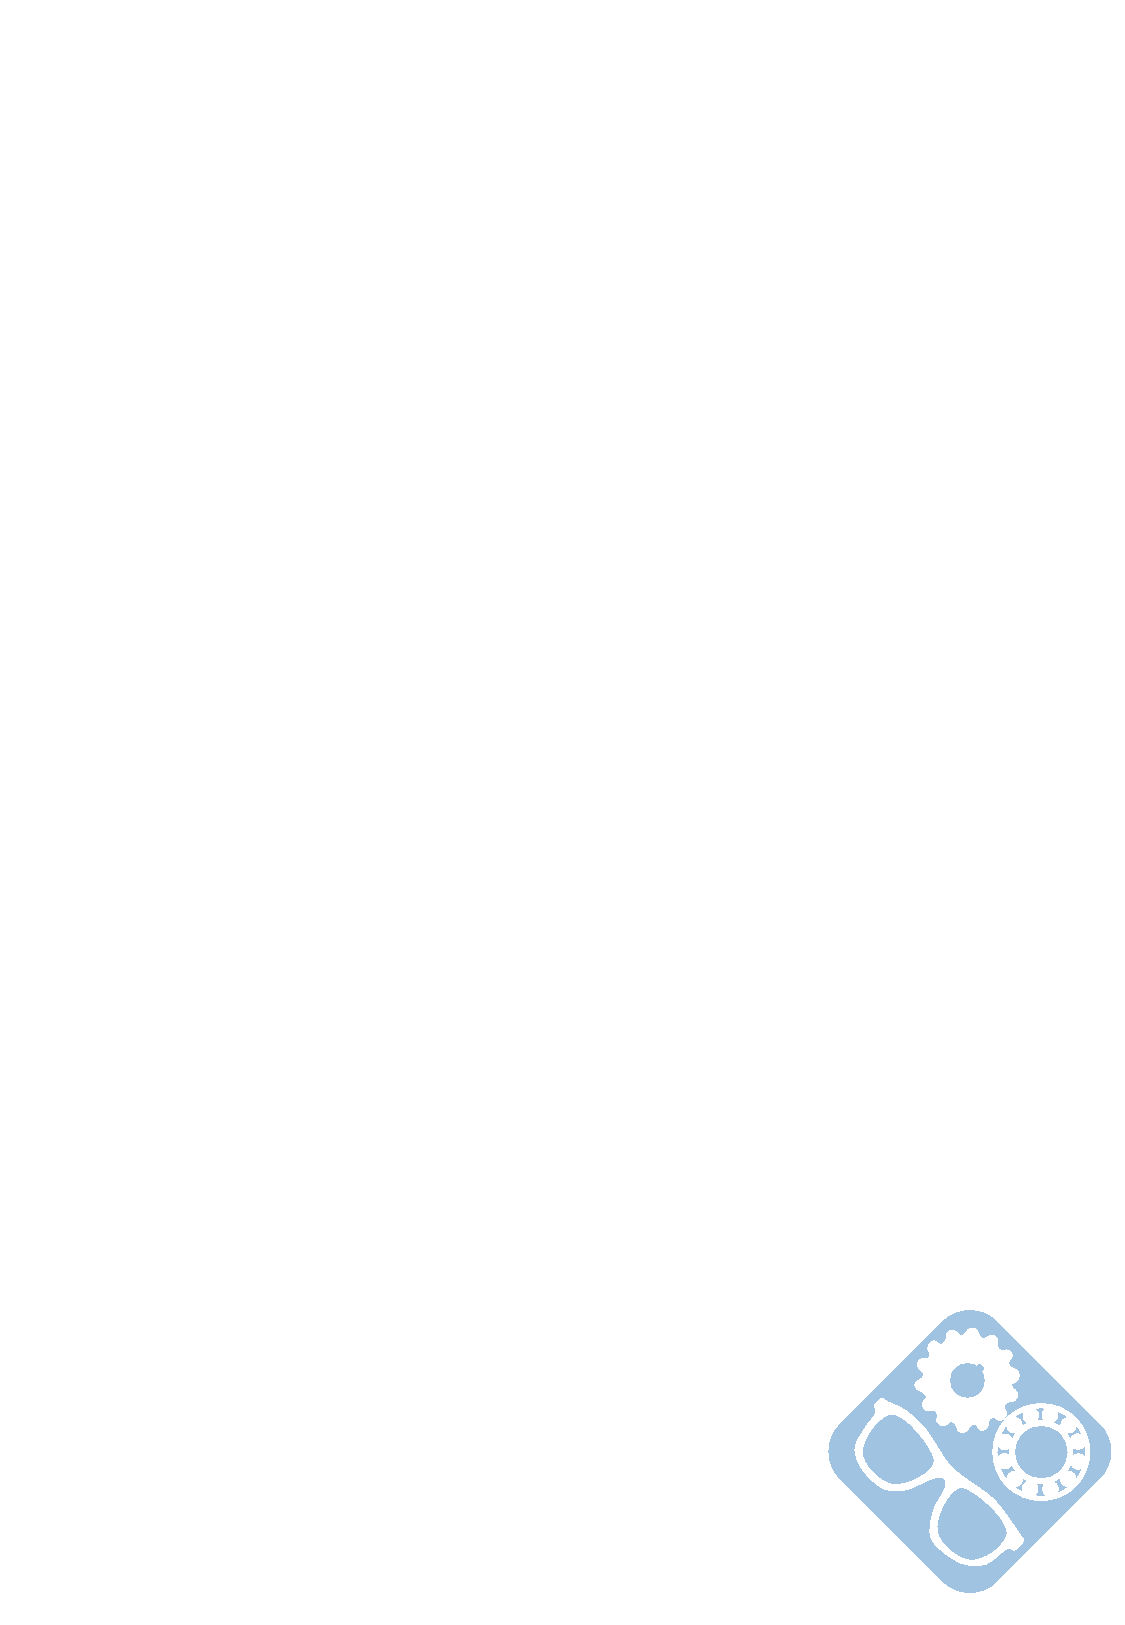
\includegraphics[width=\paperwidth,height=\paperheight,%
keepaspectratio]{../../../img/fond4}%
\end{center}
\vfill
}}}

\begin{document}

\pagestyle{empty}

\AddToShipoutPicture*{\BackgroundPic}


\includegraphics[width=2cm]{../../../img/logo}

\Huge{DS \numero - \sujet}

\vspace{1cm}

\ifdef{\prive}{\begin{center}\colorbox{danger}{\Huge{Avec Correction}}\end{center}}{}

\begin{center}
\centering\huge{PTSI}
\end{center}

\vspace{2cm}


\begin{center}
\centering\Large{\jour}
\end{center}

\vspace{2cm}

\normalsize

\tableofcontents

\newpage

\AddToShipoutPicture{\BackgroundPicdeux}

\pagestyle{fancy}

\begin{center}
\Huge \sujet
\end{center}


\normalsize


% ------------------------------------------------------------------
% Macros locales au DS02
% ------------------------------------------------------------------
\newcommand{\uu}[1]{\,\mathrm{#1}}
\newcommand{\vx}[1]{\vec{x}_{#1}}
\newcommand{\vy}[1]{\vec{y}_{#1}}
\newcommand{\vz}[1]{\vec{z}_{#1}}

\newcommand{\deuxfigures}[6]{%
\begin{figure}[ht!]
\begin{minipage}[b]{#5\linewidth}
\centering\includegraphics[width=\linewidth]{img/#1}
\caption{\label{#1}#2}
\end{minipage}\hfill
\begin{minipage}[b]{#6\linewidth}
\centering\includegraphics[width=\linewidth]{img/#3}
\caption{\label{#3}#4}
\end{minipage}
\end{figure}}
% figure non numérotée (supports de réponse et figures du corrigé) : fichier, largeur
\newcommand{\figDR}[2]{\begin{center}\includegraphics[width=#2\linewidth]{img/#1}\end{center}}

\subsection*{Contexte général}

La Philharmonie de Paris est un complexe culturel situé dans le parc de la Villette à Paris. Inaugurée en 2015, son architecture est due à Jean Nouvel. La structure en béton de 52 mètres de haut est en grande partie revêtue d'aluminium et offre un panorama sur Paris et ses alentours (figure~\ref{fig01}).

\deuxfigures{fig01}{La Philharmonie de Paris, vue extérieure (W. Beaucardet, 2016)}{fig02}{Intégration de la grande salle \og Pierre Boulez \fg{} dans le bâtiment (Atelier J. Nouvel)}{0.45}{0.52}

Parmi les nombreux espaces du bâtiment, une salle de concert de 2400 places assises, dite grande salle \og Pierre Boulez \fg{}, est principalement consacrée à la musique symphonique (figure~\ref{fig02}). Il s'agit d'une salle enveloppante (le public peut être installé à 360 degrés autour de la scène) et modulable qui peut également s'adapter à la musique de chambre, au jazz ou aux musiques du monde. C'est la disposition de la salle elle-même qui est alors modifiée pour offrir le meilleur confort visuel et auditif quel que soit le type de spectacle proposé.

\deuxfigures{fig03}{Configuration symphonique (J. Mignot, 2017)}{fig04}{Configuration ciné-concert (Ava du Parc, 2017)}{0.49}{0.49}

En configuration symphonique, les spectateurs entourent l'orchestre (figure~\ref{fig03}).

Les places situées derrière la scène, en gradins, accueillent un chœur si l'œuvre interprétée l'exige ou, le plus souvent, du public. Ces gradins arrière sont télescopiques, ce qui permet de reculer la scène et d'agrandir le parterre, une configuration utilisée pour les ciné-concerts ou les concerts de musique amplifiée par exemple (figure~\ref{fig04}). D'autre part, l'ensemble des gradins du parterre peuvent être escamotés pour accueillir le public debout à l'occasion des concerts de musiques actuelles par exemple, portant la capacité de la salle à 3\,500 places.

\subsection*{Machineries et modularité}

C'est la société AMG-Féchoz, leader français en machinerie scénique, qui a assuré la conception et la réalisation des éléments modulables de la grande salle de la Philharmonie de Paris. Ce projet a dû s'adapter aux contraintes liées à l'originalité du lieu comme le fait que la salle ne soit pas symétrique ou encore l'absence de murs porteurs à proximité des machineries. Le passage d'une configuration de salle à l'autre est en grande partie automatisé ce qui permet en pratique d'effectuer un changement complet en une journée avec un personnel limité.

\paragraph{Gradinage amovible du parterre.} Afin de passer d'une configuration assise à une configuration debout, l'ensemble des gradins du parterre (figure~\ref{fig05}) peut être retiré et remplacé par un plancher horizontal. Cette transformation est intégralement automatisée : les sièges se retournent et sont stockés sous un plancher qui peut être levé ou abaissé suivant les besoins.

\deuxfigures{fig05}{Vue frontale des gradins du parterre en configuration assise}{fig06}{Vue en coupe des gradins du parterre en configuration assise}{0.42}{0.45}

\begin{figure}[ht!]
\begin{minipage}[b]{0.55\linewidth}
\centering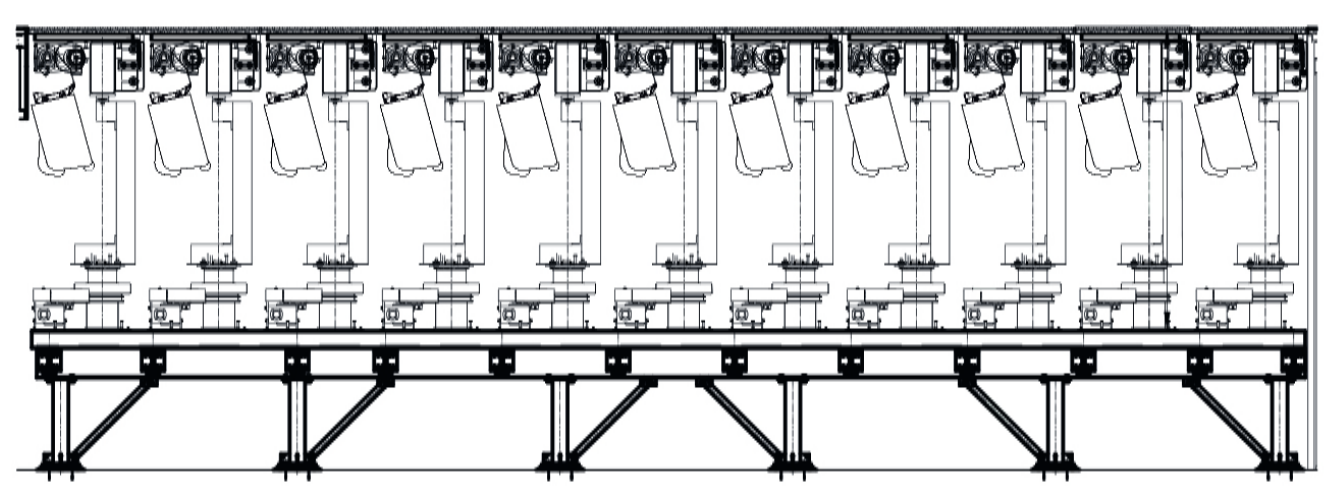
\includegraphics[width=\linewidth]{img/fig07}
\caption{\label{fig07}Vue en coupe des gradins du parterre en configuration debout (parterre escamoté)}
\end{minipage}\hfill
\begin{minipage}[b]{0.25\linewidth}
\centering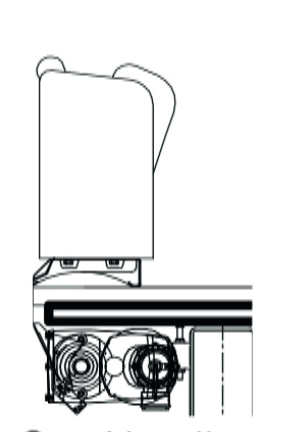
\includegraphics[width=0.4\linewidth]{img/fig08}
\caption{\label{fig08}Un siège en position levée, prêt à accueillir un spectateur}
\end{minipage}
\end{figure}

\newpage

S'il est possible de piloter indépendamment les différents rangs de sièges, c'est généralement tout le parterre qui est modifié. Les vues en coupes figure~\ref{fig06} et figure~\ref{fig07} illustrent les deux configurations extrêmes associées à deux utilisations différentes de la salle. En annexe A, la figure~\ref{fig35} permet de restituer ces gradins dans le contexte global de la salle.

\paragraph{Élévateur d'orchestre.} La scène principale est dimensionnée pour pouvoir accueillir un orchestre. Elle peut être adaptée très précisément aux spectacles donnés en fonction du nombre de musiciens présents ou de leur disposition. Elle est composée de 28 éléments de surfaces visibles figure~\ref{fig09} qui peuvent être élevés indépendamment les uns des autres (figure~\ref{fig10}) ainsi que de 2 escaliers télescopiques.

\deuxfigures{fig09}{Dessin de l'ensemble des modules composant le support d'orchestre}{fig10}{Vue 3D partielle de 4 modules pilotables indépendamment}{0.5}{0.45}

D'autres éléments modulaires tels que les gradins de la tribune télescopique à l'arrière de l'orchestre sont visibles sur les vues en coupe de l'annexe A mais ne seront pas étudiés dans ce sujet.

\subsection*{Travail à réaliser}

Après une lecture préalable du sujet complet, vous serez amené à vous intéresser à 4 parties indépendantes, elles-mêmes constituées de nombreuses questions qui peuvent être traitées séparément :
\begin{itemize}
\item la \textbf{partie I} aborde l'étude du parterre escamotable et la description temporelle d'un changement de configuration de salle ;
\item la \textbf{partie II} s'intéresse à la commande d'un couple de moteurs destinés à lever un élément de parterre ;
\item la \textbf{partie III} se sur la conception d'une partie du mécanisme.
\end{itemize}

\subsection*{Applications numériques et notations}

\textbf{Applications numériques.} Dans le domaine des Sciences Industrielles, le fait de savoir calculer et analyser les valeurs des grandeurs utiles au dimensionnement est aussi important que celui de savoir déterminer leurs expressions littérales. C'est pourquoi \textbf{une attention toute particulière sera accordée à la réalisation des applications numériques}.

Pour réaliser celles-ci sans l'usage d'une calculatrice, vous pourrez faire des approximations de bon sens, qui conduiront éventuellement à une erreur relative de quelques pourcents sur le résultat final. Par exemple, dans le calcul suivant, qui fait intervenir l'accélération de la pesanteur $g=9{,}81\uu{m\cdot s^{-2}}$, on pourra prendre :
\[
\dfrac{\pi^2}{2}\,\dfrac{100}{24}\,(5+3\cdot 10^{-2})\,g\approx \dfrac{10}{2}\times 4\times 5\times 10=1000\uu{m\cdot s^{-2}}
\]

\textbf{Notations.} 
\begin{comment}
Pour simplifier les notations dans ce sujet, le référentiel correspondant à un repère $\mathcal{R}_i$ est lui aussi désigné par $\mathcal{R}_i$. Les torseurs cinématique, cinétique et dynamique du mouvement du solide $j$ par rapport au solide $i$ (ou par rapport au référentiel $\mathcal{R}_i$ lié à celui-ci), exprimés en $A$, sont notés respectivement :
\[
\mathcal{V}(j/i)=\torseurh{\vec{\Omega}(j/i)}{\vec{V}(A,j/i)}{A},\qquad
\mathcal{C}(j/i)=\torseurh{\vec{R}_c(j/i)}{\vec{\sigma}(A,j/i)}{A}\qquad\text{et}\qquad
\mathcal{D}(j/i)=\torseurh{\vec{R}_d(j/i)}{\vec{\delta}(A,j/i)}{A}
\]
Le torseur des actions mécaniques exercées par le solide $i$ sur le solide $j$, exprimé en $A$, est noté :
\[
\mathcal{T}(i\to j)=\torseurh{\vec{F}(i\to j)}{\vec{M}(A,i\to j)}{A}
\]
\end{comment}

Les dérivées première et seconde d'une quantité $x(t)$ par rapport au temps pourront être notées indifféremment : $\dot{x}=\dfrac{dx}{dt}$ et $\ddot{x}=\dfrac{d^2x}{dt^2}$. Enfin, on notera, lorsque cela est possible, une fonction dans le domaine temporel par une lettre minuscule (e.g. $i(t)$) et sa transformée de Laplace par une lettre majuscule (soit $I(p)$).

\emph{Remarque. --- Les modélisations et valeurs numériques utilisées dans ce sujet ne sont que des illustrations du système réel et n'engagent en aucune façon la société AMG-Féchoz. Les auteurs du sujet remercient la société AMG-Féchoz pour la mise à disposition des informations et documents utilisés dans ce sujet ainsi que pour leur accord concernant leur publication.}

\newpage

%%%%%%%%%%%%%%%%%%%%%%%%%%%%%%%%%%%%%%%%%%%%%%%%%%%%%%%%%%%%%%%%%%%%%%
\section{Étude du parterre escamotable}

\textbf{Objectif.} Dans cette première partie, on étudie le passage d'un parterre en configuration debout (pas de gradin, voir figure~\ref{fig07}) à un parterre en configuration assise (figure~\ref{fig06}). Ce changement de configuration doit être rapide et sécurisé. Un extrait du cahier des charges permettant de respecter ces conditions est donné ci-dessous.

\begin{center}
\begin{tabular}{|p{3.2cm}|p{5.6cm}|p{6.4cm}|}
\hline
\textbf{Exigence} & \textbf{Critères d'appréciation} & \textbf{Niveau} \\
\hline
Changer rapidement la configuration du parterre &
$\bullet$ Durée du changement\newline $\bullet$ Automatisation du système &
$\bullet$ $<10$ min\newline $\bullet$ 100\,\% : pas de manipulation manuelle d'élément \\
\hline
Changer la configuration du parterre en toute sécurité &
$\bullet$ Contrôle et surveillance visuelle de la manœuvre\newline
$\bullet$ Information de changement de configuration\newline
$\bullet$ Absence de contact entre les éléments en mouvement &
$\bullet$ Pupitre de contrôle mobile et déplaçable en salle\newline
$\bullet$ Activation d'un signal sonore pendant toute la durée du changement de configuration\newline
$\bullet$ Un siège ne doit jamais être à moins de 10 cm de la structure ou du siège d'un autre rang en cours de manœuvre \\
\hline
\end{tabular}
\end{center}

\subsection{Structure du gradinage}

On étudiera uniquement le positionnement vertical des 11 premiers rangs de sièges du parterre. Chaque rang peut être piloté individuellement à l'aide de vérins qui permettent de le translater verticalement. Hypothèses et paramétrage du gradinage illustré figure~\ref{fig11} :
\begin{itemize}
\item[---] on numérote les rangs de 1 à 11, le 1\ier{} rang étant le plus bas et donc le plus près de la scène ;
\item[---] en configuration à plat, tous les rangs ont une hauteur identique $H_i^{init}=H^{ref}=0\uu{mm}$ et les sièges ne sont pas retournés ;
\item[---] en configuration gradinage complet, les sièges sont en position relevée et on note $H_i^{fin}$ la position finale de chaque rang $i$ dans ce contexte. Seul le premier rang est à la même hauteur que dans la configuration à plat : $H_1^{fin}=H^{ref}=0\uu{mm}$. C'est la configuration finale qui est visible figure~\ref{fig11} ;
\item[---] la différence de hauteur entre deux rangs en configuration levée est $h=200\uu{mm}$.
\end{itemize}

Lors d'un changement de configuration de salle, il est nécessaire de faire attention à l'espace disponible derrière les rangs de gradins lors d'une rotation des sièges. Sur le document réponse, question~1, deux rangs sont visibles ainsi que les positions d'un siège pendant son mouvement de rotation afin d'illustrer l'espace nécessaire lors d'un retournement.

La configuration retenue pour ce retournement est telle que : $H_i^{rot}=1300\uu{mm}$ pour le rang $i$ et $H_{i+1}^{init}=0\uu{mm}$ pour le rang suivant.

\question{Justifier par un tracé sur le document réponse qu'il n'est pas possible de retourner les sièges du rang $i$ à la hauteur $H_i^{rot}=1300\uu{mm}$ si les sièges du rang $i+1$ sont en position levée.}

Le constructeur a retenu une hauteur de sécurité $H^s=1800\uu{mm}$. Tout retournement d'un rang de sièges doit être effectué à cette hauteur. Il est indispensable que le rang situé directement derrière le rang retourné soit alors en position de référence basse $H^{ref}$.

\posetafigure{fig11}{1}{Paramétrage des 11 premiers rangs des gradins : vue en coupe en configuration assise}

\question{Calculer $H_{11}^{fin}$ en position de gradinage complet. Est-il possible d'utiliser le même mécanisme de levage pour tous les rangs ?}

\subsection{Cycle d'ouverture}

On prend l'exemple d'un cycle d'ouverture : on souhaite passer d'une configuration salle debout (parterre horizontal et sièges escamotés, figure~\ref{fig07}) à une configuration en salle assise (gradins déployés, figure~\ref{fig11}). On limitera l'étude à l'élévation des 11 premiers rangs de gradins qui sont chacun pilotés individuellement.

\begin{comment}

Le diagramme d'état associé à un cycle d'ouverture complet est donné figure~\ref{fig12}. On constate qu'il peut être interrompu à tout instant manuellement. Lors d'un changement de configuration, plusieurs machinistes surveillent visuellement le parterre pour interrompre l'opération en urgence en cas de dysfonctionnement, notamment en cas de retournement incomplet d'un ou plusieurs rangs de sièges.

On propose de lever les rangs de sièges un par un. Le diagramme d'état associé est donné figure~\ref{fig13}. Afin de calculer la durée nécessaire pour passer d'une configuration à l'autre, on fera l'hypothèse que les vérins permettent à chaque rang de monter ou descendre à une vitesse constante $v_z=1\uu{m\cdot min^{-1}}$. On notera les durées de chacun des trois états principaux du diagramme figure~\ref{fig13} de la manière suivante :
\begin{itemize}
\item[---] $T_{mep}$ la durée de l'étape de \og mise en position \fg{} d'un rang ;
\item[---] $T_i$ la durée de l'étape de \og positionnement final \fg{} du rang $i$. Cette durée dépend de la hauteur finale du rang. On introduit $T_{moy}$ la durée moyenne de cette étape. Pour simplifier les calculs, on supposera que $T_{moy}=T_6$ car le rang 6 est le rang médian dans notre étude ;
\item[---] $t_r=15\uu{s}$ la durée de retournement d'un rang de sièges.
\end{itemize}

\deuxfigures{fig12}{Diagramme d'état général d'un changement de configuration du parterre (élévation des gradins)}{fig13}{Diagramme d'état : déploiement rang par rang des gradins}{0.36}{0.60}

\question{Quelle est la durée $T_{mep}$ ? Calculer uniquement pour le rang numéro 6 la durée $T_6$ de l'étape de \og positionnement final \fg{}. On suppose que $T_{moy}=T_6$ est la durée moyenne de cette étape. En déduire le temps de déploiement total des 11 rangs de gradins et conclure vis-à-vis du cahier des charges. Toutes les applications numériques sont demandées avec un chiffre significatif.}

Le constructeur n'a pas retenu cette procédure pour modifier la configuration du parterre. Le diagramme d'état de la figure~\ref{fig14} donne la procédure retenue. Dans ce nouveau diagramme, la variable $i$ représente la parité des rangs à déplacer et non plus le numéro du rang. Les rangs de parité $i=1$ sont les rangs impairs notés $R_{P1}=\{1,3,\dots,11\}$, et les rangs de parité $i=2$ sont les rangs pairs notés $R_{P2}=\{2,4,\dots,10\}$.

\posetafigure{fig14}{0.85}{Diagramme d'état : déploiement des gradins en deux temps}

La figure~\ref{fig15} illustre la fin de cette procédure : les rangs pairs sont tous levés à la hauteur de sécurité $H^s$ et leurs sièges viennent de se retourner. On aperçoit en contrebas les sièges des rangs impairs au niveau $H^{ref}$.

\posetafigure{fig15}{0.8}{Changement de configuration du parterre : fin de la procédure}

\end{comment}

On donne ci-dessous un extrait de la procédure de changement de configuration du parterre implémentée en langage Python. Les fonctions suivantes sont utilisées :
\begin{itemize}
\item[---] \texttt{retourner(R)} : \texttt{R} est la liste des indices des rangs à retourner. Cette fonction retourne tous les rangs d'indices inclus dans \texttt{R} ;
\item[---] \texttt{deplacer(R,H)} : \texttt{R} est la liste des indices des rangs à déplacer et \texttt{H} la liste des hauteurs à atteindre. Cette fonction déplace tous les rangs d'indices \texttt{R[i]} à la position \texttt{H[i]}.
\end{itemize}

\newpage

\begin{lstlisting}[language=Python,literate={é}{{\'e}}1 {è}{{\`e}}1 {à}{{\`a}}1 {ê}{{\^e}}1]
# Procédure de changement de configuration du parterre
# Etat initial : parterre en configuration debout : gradins escamotés
# Etat final : parterre en configuration assise : gradins déployés
while not ArretUrgence :
    for i in range(1,3) : # i = 1 : rangs impairs ; i = 2 : rangs pairs
        if i == 1:
            R = [i for i in range(1,12,2)] # rangs impairs
        else :
            R = [i for i in range(2,11,2)] # rangs pairs

        # Mise en position
        Hmep = [1800]*len(R) # Hs = 1800mm
        deplacer(R,Hmep)

        # retournement de sièges
        retourner(R)

        # position de fin de cycle
        if i == 1:
            H0 = [0]*len(R)
            deplacer(R,H0)
        else:
            # Construction de Hfinal, positions finales des rangs
            ............................... 
            Rtot = [i for i in range(1,12)] # tous les rangs
            deplacer(Rtot,Hfinal)
\end{lstlisting}


\question{En 10 lignes maximum, compléter la partie manquante du code à la ligne 24 du code ci-dessus pour construire la liste nécessaire pour déplacer l'ensemble des rangs en position finale lors de l'état \og positionnement final \fg{}.}

~\

La durée d'ouverture totale du parterre est dans ce cas de l'ordre de 8 minutes et le cahier des charges est bien respecté.

\begin{comment}

%%%%%%%%%%%%%%%%%%%%%%%%%%%%%%%%%%%%%%%%%%%%%%%%%%%%%%%%%%%%%%%%%%%%%%
\section{Modélisation d'un module du gradinage d'orchestre}

\textbf{Objectif.} Dans cette partie, on s'intéresse au système de guidage du levage d'un module de la scène modulable et l'on cherche à valider les performances associées au débattement de la plateforme d'élévateur d'orchestre. La plateforme étudiée est un des modules d'orchestre visibles en figure~\ref{fig09} et figure~\ref{fig10}. On propose ci-dessous un extrait de cahier des charges lié à l'élévation de la plateforme.

\begin{center}
\begin{tabular}{|p{4cm}|p{6.2cm}|p{4.2cm}|}
\hline
\textbf{Exigence} & \textbf{Critères d'appréciation} & \textbf{Niveau} \\
\hline
Guider la translation de la scène modulable &
$\bullet$ Degré de liberté\newline $\bullet$ Débattement\newline $\bullet$ Déplacement horizontal admissible\newline $\bullet$ Vitesse nominale de levage\newline $\bullet$ Surface d'une plateforme &
$\bullet$ 1 translation\newline $\bullet$ 1200 mm\newline $\bullet$ nul\newline $\bullet$ $1\uu{m\cdot min^{-1}}$\newline $\bullet$ $12\uu{m^2}$ \\
\hline
Positionner la plateforme &
$\bullet$ Rigidité verticale\newline $\bullet$ Rigidité transversale &
$\bullet$ maximale\newline $\bullet$ maximale \\
\hline
\end{tabular}
\end{center}

\posetafigure{fig16}{0.8}{Vue globale de la structure mécanique du module de gradinage d'orchestre. On distingue les 2 pentures, les ciseaux et les 3 vérins Spiralift. Seule la partie inférieure du gradinage est étudiée (extrait de dessin technique constructeur)}

Le module de gradinage d'orchestre étudié (voir figure~\ref{fig16} et figure~\ref{fig17}) comporte deux niveaux principaux. On s'intéressera au niveau inférieur, constitué de :
\begin{itemize}
\item[---] trois vérins actionneurs de technologie \og Spiralift \fg{} : leur principe de fonctionnement, dont la connaissance n'est pas indispensable ici, est détaillé en annexe B2 ;
\item[---] deux \og pentures \fg{}, une à chaque extrémité ;
\item[---] une structure de type \og ciseaux \fg{} positionnée en bordure de plateforme pour laisser la place aux arbres d'entraînement des vérins au centre.
\end{itemize}

\posetafigure{fig17}{1}{Vues de la structure mécanique du module en positions basse et haute (extrait de dessin technique constructeur)}

\subsection{Modélisation des liaisons}

\subsubsection{Modélisation d'une penture}

On donne en annexe B1 figure~\ref{fig36} le dessin d'ensemble d'une penture. Les solides en présence sont référencés comme suit (voir détail en figure~\ref{fig18}) :
\begin{itemize}
\item[---] le bâti 0 ;
\item[---] le caisson inférieur $P_1$ et le caisson supérieur $P_2$ ;
\item[---] la plateforme 3.
\end{itemize}

\posetafigure{fig18}{0.6}{Vue annotée d'une penture}

\question{À partir du plan (détail E de la vue en coupe A-A figure~\ref{fig36}) et après avoir analysé la géométrie des contacts, proposer une modélisation simple des 2 liaisons (en parallèle) entre le bâti 0 et le caisson $P_1$.

Que dire de la liaison entre le caisson $P_2$ et plateforme 3 (détail D de la vue en coupe A-A figure~\ref{fig36}) ?

À partir du plan (détail C de la vue en coupe B-B figure~\ref{fig36}) et après avoir analysé la géométrie des contacts, proposer une modélisation simple des 4 liaisons (en parallèle) entre les deux caissons $P_1$ et $P_2$.}

\question{Compléter le schéma cinématique partiel 3D du document réponse en faisant apparaître les huit liaisons proposées.}

Cette modélisation fait apparaître un certain nombre de liaisons en parallèle.

\question{Donner (sans démonstration) la liaison équivalente entre le bâti 0 et le caisson $P_1$. La liaison entre le caisson $P_2$ et la plateforme 3 est de même type.

De même, donner (sans démonstration) la liaison équivalente entre les caissons $P_1$ et $P_2$.

Dessiner alors le schéma cinématique minimal en 2D.}

Cette modélisation sera utilisée pour l'étude du gradinage complet.

\subsubsection{Modélisation des liaisons d'un vérin}

Les vérins employés sont de technologie Spiralift. Chaque vérin $V_i$ est modélisé ici par l'ensemble de deux pièces, une tige $T_i$ en liaison glissière par rapport à un corps $C_i$. Dans un premier temps, on considère que le corps $C_i$ est en liaison encastrement avec le bâti 0 et la tige $T_i$ en liaison encastrement avec la plateforme 3 : ces liaisons encastrements sont réalisées par des montages boulonnés visibles en figure~\ref{fig39} (annexe B2).

\subsection{Validation de la cinématique de la plateforme}

Afin de vérifier la mobilité de la plateforme résultant de sa structure cinématique, nous étudierons dans un premier temps la structure constituée de deux pentures, puis celle de la structure ciseaux, avant d'étudier l'ensemble du mécanisme.

\subsubsection{Association de deux pentures}

On propose en figure~\ref{fig19} un schéma cinématique paramétré d'une penture. On note $P_1$ et $P_2$ les deux caissons, 0 le bâti et 3 la plateforme. Le mécanisme constitué de deux pentures en parallèle est détaillé figure~\ref{fig20}.

\deuxfigures{fig19}{Schéma cinématique paramétré d'une penture}{fig20}{Schéma cinématique de deux pentures en parallèle}{0.36}{0.58}

On donne les caractéristiques géométriques suivantes :
\begin{itemize}
\item[---] le bâti 0 est muni du repère $\mathcal{R}_0=(A,\vx0,\vy0,\vz0)$. Le référentiel associé est supposé galiléen ;
\item[---] le caisson inférieur $P_1$, muni du repère $\mathcal{R}_{P_1}=(A,\vx{P_1},\vy{P_1},\vz0)$, est lié au bâti 0 par une liaison pivot d'axe $(A,\vz0)$. On note $\theta_{P_1}=(\vx0,\vx{P_1})=(\vy0,\vy{P_1})$ ;
\item[---] le caisson supérieur $P_2$, muni du repère $\mathcal{R}_{P_2}=(B,\vx{P_2},\vy{P_2},\vz0)$, est lié au caisson $P_1$ par une liaison pivot d'axe $(B,\vz0)$. On note $\theta_{P_2}=(\vx{P_1},\vx{P_2})=(\vy{P_1},\vy{P_2})$ ;
\item[---] la plateforme 3, munie du repère $\mathcal{R}_3=(C,\vx3,\vy3,\vz0)$, est liée au caisson $P_2$ par une liaison pivot d'axe $(C,\vz0)$. On note $\theta_{P_3}=(\vx{P_2},\vx3)=(\vy{P_2},\vy3)$ ;
\item[---] les deux caissons $P_1$ et $P_2$ ont même longueur $L_P=1{,}3\uu{m}$ : $\overrightarrow{AB}=L_P\,\vx{P_1}$ et $\overrightarrow{BC}=L_P\,\vx{P_2}$.
\end{itemize}

\question{Déterminer (par le calcul) la liaison équivalente entre la plateforme 3 et le bâti 0 réalisée par une penture.

Indiquer (sans calculs) la liaison équivalente entre la plateforme 3 et le bâti 0 réalisée par les deux pentures en parallèle.}

La vue 3D du dessin technique figure~\ref{fig36} montre la géométrie des caissons de pentures (notées $P_1$ et $P_2$) : ce sont des caissons de tôles.

\question{Y a-t-il un intérêt cinématique à disposer de deux pentures en parallèle plutôt qu'une seule ? Deux pentures non motorisées en parallèle permettent-elles d'assurer l'horizontalité de la plateforme ?

Le débattement permis permet-il de vérifier le cahier des charges ?

Quel peut alors être l'intérêt mécanique de ces structures pentures ?}

\subsubsection{Structure ciseaux}

Une vue annotée d'une structure ciseaux est donnée figure~\ref{fig21}. Les solides en présence sont référencés comme suit :
\begin{itemize}
\item[---] le bâti 0 ;
\item[---] les barres 1 et 2 ;
\item[---] la plateforme 3 ;
\item[---] les galets $g_1$ et $g_2$.
\end{itemize}

En suivant une démarche similaire à celle menée précédemment, on modélise par une liaison pivot chacune des trois liaisons entre la plateforme 3 et la barre 2, entre la barre 1 et le bâti 0 ainsi qu'entre les barres 1 et 2. Le galet $g_1$ (resp. $g_2$) est considéré en liaison pivot avec la barre 1 (resp. 2) et en liaison glissière avec la plateforme 3 (resp. le bâti 0). Ces liaisons, respectant une symétrie plane, sont représentées sur le schéma cinématique plan paramétré de la figure~\ref{fig22}.

\deuxfigures{fig21}{Vue annotée de la structure ciseaux}{fig22}{Schéma cinématique paramétré d'une structure ciseaux}{0.38}{0.58}

On donne les caractéristiques géométriques suivantes :
\begin{itemize}
\item[---] le bâti 0 est muni du repère $\mathcal{R}_0=(H,\vx0,\vy0,\vz0)$. Le référentiel associé est supposé galiléen ;
\item[---] la barre 1, munie du repère $\mathcal{R}_1=(H,\vx1,\vy1,\vz0)$, est liée au bâti 0 par une liaison pivot d'axe $(H,\vz0)$. On note $\theta_1=(\vx0,\vx1)=(\vy0,\vy1)$ ;
\item[---] la barre 2, munie du repère $\mathcal{R}_2=(G,\vx2,\vy2,\vz0)$, est liée au bâti 0 par l'intermédiaire d'un galet $g_2$ : le galet $g_2$ est en liaison pivot d'axe $(G,\vz0)$ avec la barre 2 et en liaison glissière de direction $\vx0$ avec le bâti 0. On note $\theta_2=(\vx0,\vx2)=(\vy0,\vy2)$ ;
\item[---] les deux barres 1 et 2 sont liées entre elles par une liaison pivot d'axe $(F,\vz0)$ ;
\item[---] la plateforme 3, munie du repère $\mathcal{R}_3=(E,\vx3,\vy3,\vz0)$, est liée à la barre 2 par une liaison pivot d'axe $(E,\vz0)$ ainsi qu'à la barre 1 par l'intermédiaire d'un galet $g_1$ : le galet $g_1$ est en liaison pivot d'axe $(D,\vz0)$ avec la barre 1 et en liaison glissière de direction $\vx0$ avec la plateforme 3. On note $\theta_3=(\vx1,\vx3)=(\vy1,\vy3)$ ;
\item[---] les deux barres 1 et 2 ont même longueur, notée $L_b$ : $\overrightarrow{HD}=2\overrightarrow{HF}=L_b\,\vx1$ et $\overrightarrow{GE}=2\overrightarrow{GF}=L_b\,\vx2$, avec $L_b=2\uu{m}$ ;
\item[---] on note $\overrightarrow{HG}=\lambda(t)\,\vx0$.
\end{itemize}

\question{Quelle est la particularité géométrique du quadrilatère $HEDG$ ?

En déduire sans calcul la caractéristique du mouvement de la plateforme 3 par rapport au bâti 0.

Quel est l'intérêt cinématique d'une structure ciseaux ?}

\question{Écrire les fermetures géométriques des deux chaînes $(0-1-2-g_2)$ et $(3-g_1-1-2)$ et exprimer $\overrightarrow{ED}$ en fonction d'un unique paramètre ainsi que $\theta_2$ en fonction de $\theta_1$.}

\question{Quel encombrement horizontal prévoir pour une telle structure ciseaux de débattement vertical imposé ? Quelle solution visible en figure~\ref{fig16} et figure~\ref{fig17} est utilisée au niveau supérieur et pour quelle raison ?}

\question{Exprimer les torseurs cinématiques $\mathcal{V}(1/0)$, $\mathcal{V}(2/1)$, $\mathcal{V}(2/g_2)$ et $\mathcal{V}(g_2/0)$. Écrire la fermeture cinématique de chaîne $0-1-2-g_2$. En déduire l'équation vectorielle de vitesse au point $F$.}

On pose $V_{30}(t)$ la vitesse verticale de la plateforme, définie par $\left.\dfrac{d\overrightarrow{HE}}{dt}\right|_0=V_{30}(t)\,\vy0$.

\question{Exprimer $V_{30}(t)$ et $\dot{\lambda}(t)$ en fonction de $\dot{\theta}_1(t)$ et de la géométrie du système. En déduire une relation liant $\dot{\lambda}(t)$ et $V_{30}(t)$ indépendante de $\dot{\theta}_1(t)$.}

Ce résultat permet de dimensionner les liaisons glissières par galet (dimensionnement non réalisé ici).

\subsection{Modélisation globale}

\subsubsection{Première modélisation}

On s'intéresse à présent à l'intégralité d'un module du gradinage d'orchestre. On ne considérera ici que deux vérins afin d'alléger la modélisation, le vérin central est donc volontairement omis. Ainsi, pour cette première modélisation, on propose le schéma cinématique global de la figure~\ref{fig23}.

\posetafigure{fig23}{1}{Schéma cinématique d'un module du gradinage d'orchestre}

\question{Déterminer le degré d'hyperstatisme de cette modélisation en considérant que le problème est tridimensionnel.}

\question{Déterminer le degré d'hyperstatisme de cette modélisation en considérant maintenant que le problème est bidimensionnel. Comment expliquer les différences avec la valeur d'hyperstatisme en 3D calculée à la question précédente ?}

\subsubsection{Évolution de la modélisation vers un isostatisme}

Le constructeur s'assure du bon positionnement des liaisons dans les pentures et ciseaux (par un usinage laser, des jeux et positionnements réglés au montage, \dots) de façon à ce que l'hyperstatisme associé au modèle 3D lié aux liaisons pivots de cette modélisation ne pose pas de problème. Ainsi par la suite on pourra se contenter d'analyser le problème en 2D dans le plan médian.

Le modèle étudié précédemment implique des sollicitations de cisaillement des vérins (reprise d'efforts transverses dans les liaisons glissières) qui sont à proscrire car ils ne sont pas conçus pour y résister. Il est donc nécessaire de s'assurer de réaliser un montage isostatique en laissant du jeu en rotation dans la réalisation de la liaison entre la tige de vérin $T_i$ avec la plateforme supérieure 3.

\question{Quel composant visible en annexe B2 figure~\ref{fig39} permet de justifier la possibilité d'une rotation dans la liaison de chaque tige de vérin $T_i$ avec la plateforme supérieure 3 ?}

Un composant équivalent est également présent entre chaque corps de vérin $C_i$ et le bâti 0. On peut ainsi modéliser ces liaisons par des sphériques (en modélisation 3D) ou pivots (en modélisation 2D) avec frottements. Le schéma cinématique isostatique plan associé est proposé en figure~\ref{fig24}. Cette modélisation assure que les vérins ne reprennent que des efforts verticaux.

\posetafigure{fig24}{1}{Schéma cinématique du gradinage d'orchestre isostatique en étude plane}

\subsection{Reprise des actions mécaniques}

\textbf{Objectif.} Déterminer le rôle mécanique de chaque structure composant le mécanisme de levage.

\subsubsection{Isolement des éléments d'une penture}

On trouvera dans le document réponse un schéma cinématique partiel rappelant la cinématique d'une penture paramétrée en figure~\ref{fig19}.

\question{Par un isolement simple mais rigoureusement justifié, sous l'hypothèse de problème plan, donner la direction du glisseur appliqué par le caisson inférieur $P_1$ sur le caisson supérieur $P_2$. Par un raisonnement similaire, donner la direction du glisseur appliqué par le caisson supérieur $P_2$ sur le caisson inférieur $P_1$.

Indiquer ces directions sur le schéma cinématique partiel du document réponse.

En déduire la valeur de l'effort transmis entre les deux caissons $P_1$ et $P_2$.

Conclure sur la capacité d'une penture à transmettre un effort entre la plateforme 3 et le bâti 0 dans le plan $(O,\vx0,\vy0)$.}

\subsubsection{Bilan}

\question{Par des raisonnements similaires qu'il n'est pas nécessaire de préciser, indiquer dans le tableau du document réponse quelle(s) structure(s) permet(tent) de transmettre chacune des actions mécaniques entre la plateforme 3 et le bâti 0 : $F_X$ (effort suivant $\vx0$), $F_Y$ (effort suivant $\vy0$), $F_Z$ (effort suivant $\vz0$) et $M_X$ (moment suivant $\vx0$), $M_Y$ (moment suivant $\vy0$), $M_Z$ (moment suivant $\vz0$). On entourera les cas correspondants.

Conclure sur le choix de l'association de pentures, ciseaux et vérins.}

%%%%%%%%%%%%%%%%%%%%%%%%%%%%%%%%%%%%%%%%%%%%%%%%%%%%%%%%%%%%%%%%%%%%%%
\section{Dimensionnement des actionneurs}

\textbf{Objectif.} Dans cette partie, on s'intéresse au dimensionnement des actionneurs du système de levage d'un module du gradinage d'orchestre. Un extrait de cahier des charges lié à l'élévation de la scène modulable est donné ci-dessous. On se propose d'utiliser une approche énergétique dans le référentiel terrestre, supposé galiléen, auquel on associe le repère $\mathcal{R}_0=(A,\vx0,\vy0,\vz0)$ pour déterminer l'effort maximal à développer par chaque vérin.

\begin{center}
\begin{tabular}{|p{3.2cm}|p{6.6cm}|p{4.6cm}|}
\hline
\textbf{Exigence} & \textbf{Critères d'appréciation} & \textbf{Niveau} \\
\hline
Lever la scène modulable &
$\bullet$ Débattement\newline $\bullet$ Vitesse nominale de levage\newline $\bullet$ Surface d'une plateforme\newline $\bullet$ Effort surfacique à fournir en dynamique &
$\bullet$ 1200 mm\newline $\bullet$ $1\uu{m\cdot min^{-1}}$\newline $\bullet$ $12\uu{m^2}$\newline $\bullet$ $\rho_D=250\uu{daN\cdot m^{-2}}$ \\
\hline
\end{tabular}
\end{center}

On se base sur la modélisation simplifiée proposée en figure~\ref{fig25}, où sont pris en compte et représentés seulement :
\begin{itemize}
\item[---] une des deux pentures (caissons notés $P_1$ et $P_2$) ;
\item[---] la structure ciseaux (barres notées 1 et 2 et galets $g_1$ et $g_2$) ;
\item[---] un des trois vérins (corps noté $C_1$ et tige notée $T_1$) ;
\item[---] la plateforme 3.
\end{itemize}

\posetafigure{fig25}{0.8}{Schéma cinématique du gradinage d'orchestre simplifié}

On précise les hypothèses suivantes :
\begin{itemize}
\item[---] on note $\Sigma=\{P_1\,;P_2\,;1\,;2\,;g_1\,;g_2\,;3\}$ l'ensemble mobile isolé, considéré à masse constante ;
\item[---] on note $m_P=160\uu{kg}$ la masse d'un caisson de penture, de longueur $L_P=1{,}3\uu{m}$ ;
\item[---] on considère les masses et inerties des barres et galets de la structure ciseaux négligeables devant celles des caissons de pentures ;
\item[---] la charge dynamique correspondant à la masse surfacique de la plateforme 3 est $\rho_D=250\uu{daN\cdot m^{-2}}$. Le cahier des charges stipule que le levage doit s'effectuer plateforme vide donc sans masse additionnelle (aucune personne, pas de piano ni de décor, \dots). On considère que cette plateforme 3 est rectangulaire, sa longueur (suivant $\vx0$) est notée $L_3$ et sa largeur (suivant $\vz0$) $\ell_3$ ;
\item[---] on suppose les liaisons parfaites ;
\item[---] on modélise l'action motrice dans le vérin par un glisseur $\mathcal{T}(T_1\to3)=\torseurh{F_v\,\vy0}{\vec{0}}{Q_1}$ où $Q_1$ est le centre de liaison de la tige de vérin $T_1$ avec la plateforme 3 ;
\item[---] $\delta(t)=\overrightarrow{AC}\cdot\vy0=\overrightarrow{O_1Q_1}\cdot\vy0$ est l'élévation de la plateforme 3, égal à l'allongement d'un vérin.
\end{itemize}

\subsection{Calcul des énergies cinétiques en jeu}

Le dessin d'ensemble donné en annexe B1 figure~\ref{fig36} précise la géométrie 3D d'une penture, constituée de deux caissons articulés. On en propose un extrait 2D annoté en figure~\ref{fig26}. On remarquera que $A$, $G_{P_1}$ et $B$ ne sont pas alignés.

\posetafigure{fig26}{0.75}{Vue annotée d'une penture dans le plan médian de normale $\vz0$}

\question{À partir de l'analyse de ses caractéristiques géométriques, préciser la forme de la matrice d'inertie d'un caisson de penture $P_1$ au centre de gravité $G_{P_1}$ dans la base $\mathcal{B}_1=(\vx{P_1},\vy{P_1},\vz0)$, notée $\mathcal{I}(G_{P_1},P_1)$.}

Par la suite, on simplifiera la géométrie en considérant que $G_{P_1}$ (resp. $G_{P_2}$) est au milieu de $\overrightarrow{AB}$ (resp. $\overrightarrow{BC}$) : $\overrightarrow{AG_{P_1}}=\dfrac{\overrightarrow{AB}}{2}=\dfrac{L_P}{2}\vx{P_1}$ et $\overrightarrow{BG_{P_2}}=\dfrac{\overrightarrow{BC}}{2}=\dfrac{L_P}{2}\vx{P_2}$. La modélisation cinématique des pentures dans ce cas de translation verticale de la plateforme est schématisée et paramétrée en figure~\ref{fig27}.

On donne $I_P=26\uu{kg\cdot m^2}$ le moment d'inertie autour de l'axe principal d'inertie $(G_{P_i},\vz0)$ d'un caisson de penture $P_i$ ($i=1$ ou 2).

\posetafigure{fig27}{0.45}{Schéma cinématique partiel détaillant la position de $G_{P_1}$ et $G_{P_2}$}

\question{Donner l'énergie cinétique de la plateforme 3 dans son mouvement par rapport au bâti 0, notée $E_c(3/0)$, en fonction de $\dot{\delta}(t)$ et des paramètres de masse et de géométrie.}

\question{Que dire de l'énergie cinétique des éléments de la structure ciseaux dans leurs mouvements par rapport au bâti 0 ?}

\question{Préciser les éléments de réduction du torseur cinétique $\mathcal{C}(P_1/0)$ en son centre de gravité $G_{P_1}$.

Déterminer l'énergie cinétique du caisson de penture $P_1$ dans son mouvement par rapport au bâti 0, notée $E_c(P_1/0)$, en fonction de $\dot{\theta}_{P_1}$ et des paramètres de masse et de géométrie.}

\question{Préciser les éléments de réduction du torseur cinétique $\mathcal{C}(P_2/0)$ en son centre de gravité $G_{P_2}$.

Déterminer l'énergie cinétique du caisson de penture $P_2$ dans son mouvement par rapport au bâti 0, notée $E_c(P_2/0)$, en fonction de $\dot{\theta}_{P_1}$, $\dot{\theta}_{P_2}$ et des paramètres de masse et de géométrie.}

\subsection{Calcul des puissances en jeu}

\question{Déterminer la puissance de l'action motrice développée par le vérin 1 : $\mathcal{P}_{T_1\to3/0}$.

Que dire de la puissance des actions mécaniques intérieures à $\Sigma$, notée $\mathcal{P}_{int}$ ?}

\question{Déterminer la puissance des actions de pesanteur appliquées à $\Sigma$ : $\mathcal{P}_{Pes\to\Sigma/0}$ en fonction de $\dot{\delta}$, $\dot{\theta}_{P_1}$, $\dot{\theta}_{P_2}$, et des paramètres de masse et de géométrie.}

\subsection{Loi de mouvement}

Dans un premier temps, afin d'obtenir l'expression de $F_v$ en fonction uniquement des paramètres de position $\delta$ et de vitesse $\dot{\delta}$, il est nécessaire de relier $\theta_{P_1}$ et $\theta_{P_2}$ à ce paramètre d'élévation $\delta$.

\question{En précisant la relation vectorielle de fermeture utilisée, prouver que $\delta=2L_P\sin(\theta_{P_1})$ et $\theta_{P_2}=\pi-2\theta_{P_1}$.}

\question{Citer rigoureusement le théorème permettant d'obtenir la loi de mouvement, à savoir l'expression de l'effort moteur $F_v$ en fonction des masse(s), longueur(s) et inertie(s) en jeu et des paramètres de mouvement $\delta(t)$ et $\dot{\delta}(t)$.}

Pour alléger les calculs, on se limite à la prise en compte des termes prépondérants, à savoir :
\begin{itemize}
\item[---] les énergies cinétiques des éléments autres que la plateforme 3 sont négligées : $E_c(\Sigma/0)=E_c(3/0)$ ;
\item[---] les puissances autres que celle de la pesanteur sur la plateforme 3 et celles des motorisations des 3 vérins sont négligées : $\mathcal{P}_{ext\to\Sigma/0}=\mathcal{P}_{Pes\to3/0}+3\,\mathcal{P}_{T_1\to3/0}$.
\end{itemize}

\question{Détailler les calculs permettant d'obtenir la loi de mouvement ainsi simplifiée, à savoir l'expression de l'effort moteur $F_v$ en fonction des masse(s), longueur(s) et inertie(s) en jeu et des paramètres de mouvement $\delta(t)$ et $\dot{\delta}(t)$.}

On trouve numériquement l'effort maximal à développer par chaque vérin, $F_v^{max}=1{,}5\cdot10^4\uu{N}$, ce qui permet de choisir le modèle de motorisation des vérins Spiralift.


\end{comment}
\newpage
%%%%%%%%%%%%%%%%%%%%%%%%%%%%%%%%%%%%%%%%%%%%%%%%%%%%%%%%%%%%%%%%%%%%%%
\section{Structure et dimensionnement d'une motorisation double}

\textbf{Objectif.} L'objectif de cette dernière partie est de vérifier que la commande de la motorisation du levage d'une plateforme mobile à l'aide de deux moteurs répond bien aux exigences du cahier des charges. Un extrait de cahier des charges associé au dimensionnement de l'une des plateformes supportant une rangée de sièges du parterre et de sa commande est donné ci-dessous.

\begin{center}
\begin{tabular}{|p{3.4cm}|p{7cm}|p{4.2cm}|}
\hline
\textbf{Exigence} & \textbf{Critères d'appréciation} & \textbf{Niveau} \\
\hline
Supporter la plateforme chargée et compenser les effets dynamiques &
$\bullet$ Effort surfacique à fournir en dynamique &
$\bullet$ $\rho_D=250\uu{daN\cdot m^{-2}}$ \\
\hline
Contrôler la vitesse de montée de la plateforme &
$\bullet$ Vitesse en régime permanent pour un chargement équivalent sur l'axe $C_r=-10\uu{N\cdot m}$\newline
$\bullet$ Dépassement pour une consigne échelon\newline
$\bullet$ Temps de réponse &
$\bullet$ $>80\,\%$ de la vitesse nominale $N=1400\uu{tr\cdot min^{-1}}$\newline
$\bullet$ Aucun\newline
$\bullet$ $<0{,}1\uu{s}$ \\
\hline
Positionner verticalement la plateforme &
$\bullet$ Durée d'élévation d'une plateforme sur 2000 mm\newline
$\bullet$ Erreur statique pour un échelon de 2000 mm\newline
$\bullet$ Erreur statique pour un chargement $C_r=-10\uu{N\cdot m}$\newline
$\bullet$ Dépassement\newline
$\bullet$ Marge de phase\newline
$\bullet$ Marge de gain &
$\bullet$ $<1$ min\newline
$\bullet$ $<1$ mm\newline
$\bullet$ $<1$ mm\newline
$\bullet$ Aucun\newline
$\bullet$ $\geqslant 60^\circ$\newline
$\bullet$ $\geqslant 15\uu{dB}$ \\
\hline
\end{tabular}
\end{center}

La motorisation d'une plateforme est illustrée figure~\ref{fig28}. On peut visualiser :
\begin{itemize}
\item[---] deux motoréducteurs-freins à chaque extrémité de la plateforme ;
\item[---] après un éventuel renvoi d'angle, les motoréducteurs-freins sont accouplés à des arbres de transmission via un joint de cardan. Ces arbres tournent tous à la même vitesse : les vitesses de rotation des moteurs accouplés à ce jeu d'arbres de transmission sont donc identiques pour des raisons mécaniques ;
\item[---] un ensemble de vérins Spiralift (jusqu'à 5 suivant les plateformes). Les arbres de transmission permettent de fournir à chaque vérin la même vitesse de rotation d'entrée. Une transmission roue et vis sans fin transmet ensuite localement ce mouvement de rotation en entrée de chaque vérin (voir annexe B2 figure~\ref{fig38}).
\end{itemize}

\posetafigure{fig28}{1}{Vue partielle de la motorisation d'une plateforme mobile. Seules les extrémités de la plateforme choisie sont visibles}

\newpage

\subsection{Modélisation de la double motorisation}

On modélisera de manière simplifiée chaque ensemble motoréducteur-frein par une machine à courant continu présentée dans le schéma-blocs de la figure~\ref{fig29}.

\posetafigure{fig29}{0.8}{Schéma-blocs de la modélisation retenue pour un moteur}

On donne les paramètres suivants :
\begin{itemize}
\item[---] $U_{eq}$ la tension continue d'alimentation du moteur, $\Omega_m$ la vitesse de rotation de l'arbre moteur et $C_r<0$ le couple résistant exercé sur cet arbre ;
\item[---] $R_{eq}=25\uu{\Omega}$ la résistance équivalente du circuit d'entrée ;
\item[---] $J=1{,}0\cdot10^{-3}\uu{kg\cdot m^2}$ l'inertie de l'arbre moteur ;
\item[---] $f=0{,}01\uu{N\cdot m\cdot s\cdot rad^{-1}}$ le coefficient de frottement visqueux ;
\item[---] $K_{eq}=3\uu{N\cdot m\cdot A^{-1}}$ la constante de couplage ;
\item[---] on négligera l'inductance du circuit.
\end{itemize}

\question{Donner la fonction de transfert équivalente de ce moteur $H(p)=\dfrac{\Omega_m(p)}{U_{eq}(p)}$ en l'absence de couple résistant ($C_r(p)=0$).}

\question{Déterminer les coefficients caractéristiques de $H(p)$ et faire l'application numérique.}

On a en pratique deux motoréducteurs montés sur le même arbre. On néglige pour l'instant la présence du réducteur et on propose figure~\ref{fig30} une modélisation de l'accouplement de deux moteurs sur le même arbre. Des moteurs identiques ont été retenus, on néglige les éventuelles légères différences entre leurs caractéristiques et on note $R$ et $K$ leurs résistances et constantes de couplage équivalentes.

\posetafigure{fig30}{0.7}{Schéma-blocs de la modélisation retenue pour deux moteurs accouplés au même arbre}

\question{Montrer qu'en l'absence de couple résistant ($C_r(p)=0$) ce schéma-blocs est équivalent à celui d'une unique machine à courant continu telle que présentée figure~\ref{fig29}. On identifiera $K_{eq}$ et $R_{eq}$ en fonction de $K$ et $R$.}

\question{Que deviennent ces valeurs en cas de panne d'un moteur ? C'est à dire lorsque $K=0$ pour un des deux moteurs seulement. Que deviennent $K_{eq}$ et $R_{eq}$ et comment le fonctionnement général du système est-il impacté ?}

\subsection{Contrôle de la vitesse}

Aucun asservissement en vitesse n'est utilisé pour commander les moteurs : c'est la position qui sera asservie pour placer les plateformes à la hauteur désirée. On se contente lors d'un mouvement de lever de soumettre les moteurs à leur tension maximale $U_M=540\uu{V}$. Les tensions d'entrée des deux moteurs sont rigoureusement identiques comme indiqué figure~\ref{fig30}. Les critères et niveaux de performances attendus en terme de vitesse sont ceux de l'exigence \og Contrôler la vitesse de montée de la plateforme \fg{} du cahier des charges ci-dessus.

La vitesse du moteur est toujours définie à partir du schéma-blocs équivalent donné figure~\ref{fig29} et on ne néglige plus à présent le couple résistant.

\question{Déterminer le temps de réponse à 5\,\% de ce système. L'exigence de rapidité est-elle respectée ? Qu'en est-il de celle associée à la présence de dépassement ?}

~\

On introduit les constantes suivantes qui peuvent servir à simplifier l'application numérique demandée à la question suivante :
\[
K_v=\dfrac{K_{eq}}{R_{eq}f+K_{eq}^2}\approx0{,}3\uu{rad\cdot s^{-1}\cdot V^{-1}}\qquad\qquad
K_{pert}=\dfrac{R_{eq}}{R_{eq}f+K_{eq}^2}\approx3\uu{rad\cdot s^{-1}\cdot(N\cdot m)^{-1}}
\]

\question{Montrer, à partir de la figure~\ref{fig29}, que $\Omega_m(p)$ peut s'écrire sous la forme $$\Omega_m(p)=H_1(p)\cdot U_{eq}(p)+H_2(p)\cdot C_r(p)$$ Mettre $H_1(p)$ et $H_2(p)$ sous la forme canonique.}

\question{Pour une tension d'entrée maximale $U_{eq}=U_M=540\uu{V}$ et un chargement maximal $C_r=-10\uu{N\cdot m}$, quelle est la vitesse de rotation du moteur en régime permanent ? Le cahier des charges est-il respecté ?}

~\

Lors d'une utilisation normale du système, le couple équivalent ramené sur l'axe des moteurs est de l'ordre de $7\uu{N\cdot m}$, ce qui leur permet de tourner à une vitesse proche de la vitesse nominale.

\subsection{Asservissement en position}

Contrairement à la vitesse, il est nécessaire de contrôler la position finale avec précision. Les critères associés sont ceux de l'exigence \og Positionner verticalement la plateforme \fg{} du cahier des charges ci-dessus. L'asservissement de la hauteur $Z(p)$ d'une plateforme est modélisé par le schéma-blocs donné figure~\ref{fig31}. 

\posetafigure{fig31}{1}{Schéma-blocs de la modélisation retenue pour l'asservissement en position de la plateforme}

\newpage

On y retrouve les blocs suivants :
\begin{itemize}
\item[---] le codeur branché directement sur l'arbre moteur et son convertisseur ; il possède une résolution élevée et on le modélisera par un capteur de gain unitaire $K_{capt}=1\uu{V\cdot rad^{-1}}$ ;
\item $C_z(p)$ le bloc correcteur de l'asservissement en position ;
\item un bloc d'adaptation de gain $K_{adapt}$ ;
\item le réducteur des groupes motoréducteurs de rapport de réduction $r_1=\frac13$ ;
\item le rapport de réduction $r_2$ associé à la transmission par roue et vis sans fin entre l'arbre à cardan et les vérins ;
\item le rapport de réduction $r_3$ de la transmission par engrenage en entrée du vérin ;
\item le vérin Spiralift dont le pas vaut $pas=50\uu{mm\cdot tour^{-1}}$ ;
\item une saturation en amont de la boucle de vitesse qui évite d'imposer une tension supérieure à $U_M=540\uu{V}$. Elle est visible figure~\ref{fig33} mais sera négligée dans un premier temps.
\end{itemize}

\question{Donner l'expression du gain $K_{adapt}$ à partir des fonctions de transfert des autres blocs du schéma de la figure~\ref{fig31} afin que l'écart $\varepsilon(p)$ soit bien nul lorsque la consigne est atteinte.}

~\

Le modèle du moteur équivalent a été étudié dans la partie précédente. On cherche dans un premier temps à vérifier les exigences de précision.

On retient une correction proportionnelle : $C_z(p)=K_p$.

Quels que soient les résultats obtenus dans la partie précédente, on considère que, sans chargement, le moteur équivalent est modélisé par la fonction de transfert suivante :
\[
H_v(p)=\dfrac{K_v}{1+\tau_vp}\qquad\text{avec } K_v=0{,}3\uu{rad\cdot s^{-1}\cdot V^{-1}}\text{ et }\tau_v=3\uu{ms}.
\]
Le modèle complet du moteur se met alors sous la forme simplifiée présentée figure~\ref{fig32} avec $K_{pert}=3\uu{rad\cdot s^{-1}\cdot(N\cdot m)^{-1}}$.

\posetafigure{fig32}{0.5}{Schéma-blocs de la modélisation du moteur équivalent}

On pose également $r=r_1r_2r_3\dfrac{pas}{2\pi}=0{,}5\uu{mm\cdot rad^{-1}}$.

\question{Déterminer et mettre sous la forme canonique la fonction de transfert en boucle ouverte $FTBO(p)|_{Cr(p)=0}=\dfrac{M(p)}{\varepsilon(p)}$. Donner sa classe et son ordre.}

\question{Montrer que :
\[
Z(p)=\dfrac{Z_c(p)+\dfrac{K_{pert}\cdot r}{K_v\cdot K_{capt}\cdot K_p}\cdot C_r(p)}{1+\dfrac{1}{K_v\cdot K_{capt}\cdot K_p}\cdot p+\dfrac{\tau_v}{K_v\cdot K_{capt}\cdot K_p}\cdot p^2}
\]}


\question{Donner littéralement l'expression de la valeur maximale de $K_p$ permettant de respecter le critère de dépassement.}

\question{Donner littéralement l'expression de la valeur minimale de $K_p$ permettant de respecter le critère d'erreur statique pour un chargement $C_r$ donné.}

Pour la suite, on retient la valeur $K_p=100$ qui respecte les deux critères précédents et on pose : $$FTBO(p)=\dfrac{K_p\cdot K_v\cdot K_{capt}}{p\cdot (1+\tau_v\cdot p)}$$.

Elle sera décomposée comme suit :
$$FTBO_1(p)=\dfrac{K_v}{1+\tau_v\cdot p}\ et\ FTBO_2(p)=\dfrac{K_p\cdot K_{capt}}{p}$$.

\question{Tracer sur le document réponse le diagramme de Bode asymptotique de la fonction de transfert $FTBO_1$. On fera apparaître les points particuliers, notamment la pulsation de cassure $\omega_c$.}

\question{Tracer sur le document réponse le diagramme de Bode asymptotique de la fonction de transfert $FTBO_2$. On fera apparaître les points particuliers, notamment la pulsation de coupure à 0\,dB (valeur de $\omega$ pour laquelle le Gain(dB) vaut 0) notée $\omega_{0dB}$ dont on donnera les valeurs numériques avec 1 chiffre significatif.}

\question{Tracer sur le document réponse le diagramme de Bode asymptotique de la fonction de transfert $FTBO$. Justifier les constructions.}

\newpage

\posetafigure{fig33}{0.7}{Positionnement de la saturation dans le schéma-blocs complet du système}

Une simulation numérique incluant la saturation en amont du moteur (figure~\ref{fig33}) donne le résultat présenté figure~\ref{fig34}. Un échelon d'entrée de 2000 mm ainsi qu'un chargement de $-10\uu{N\cdot m}$ ont été imposés à l'instant initial.

\posetafigure{fig34}{0.9}{Évolution de la hauteur de l'élément de parterre en fonction du temps : réponse à un échelon d'entrée de 2000 mm à l'instant $t=0$ sous chargement équivalent de $-10\uu{N\cdot m}$}

\question{Sur quelle performance du cahier des charges la saturation influe-t-elle ? Conclure quant au respect du cahier des charges complet.}

\section{Conception du système d'articulation}

\question{Colorier sur le document, les classes d'équivalence de la penture de la plateforme orchestre. Le bâti (pièce qui ne bouge pas) devra être laissé en blanc (sans coloriage).}

\question{Représenter sur le document réponse la pièce 5330-15-71-008 seule selon 3 vues (droite, gauche et face), il faudra s'adapter aux axes existants sur le document réponse.}


%%%%%%%%%%%%%%%%%%%%%%%%%%%%%%%%%%%%%%%%%%%%%%%%%%%%%%%%%%%%%%%%%%%%%%
\clearpage
\section*{Annexe A}

\posetafigure{fig35}{0.95}{Grande salle en configuration symphonique (en haut) et en configuration ciné-concert (en bas)}

\clearpage
\section*{Annexe B1 : dessin d'ensemble d'une penture}

\posetafigure{fig36}{.8}{Dessin technique de définition d'une penture}

\clearpage
\section*{Annexe B2 : description d'un vérin Spiralift}

Le vérin Spiralift, développé par la société GALA System, est un vérin de levage compact composé de deux bandes en acier inoxydable qui forment une colonne rigide capable de supporter des charges suivant son axe. La bande horizontale, stockée empilée dans la partie basse du vérin (voir figure~\ref{fig38}), est déployée en hélice par un mécanisme de déploiement. La bande circulaire, stockée comprimée radialement, se déploie et vient se positionner dans l'interstice de cette hélice, créant la colonne rigide (voir figure~\ref{fig37}). La tige de ce vérin est donc assemblée lors de l'élévation et désassemblée lors de la descente. La compacité du vérin est un atout incomparable pour le levage d'une scène. Par exemple le modèle HD9 possède 60 cm de hauteur en position fermée pour une course de 6 m.

\posetafigure{fig37}{0.5}{Vue 3D de l'ensemble d'un vérin Spiralift}

\clearpage

\posetafigure{fig38}{1}{Vue 3D en coupe de la partie inférieure d'un vérin Spiralift}

\posetafigure{fig39}{0.9}{Détail de la liaison d'une tige de vérin $T_i$ avec la plateforme supérieure}

\clearpage

\posetafigure{log}{1}{Tracé de la fonction $f(x)=log(x)$}


%\finsujet{public}
\finsujet{}

\clearpage

\debutcor

\newcommand{\ouic}{\fbox{oui}}
\newcommand{\nonc}{\fbox{non}}

%%%%%%%%%%%%%%%%%%%%%%%%%%%%%%%%%%%%%%%%%%%%%%%%%%%%%%%%%%%%%%%%%%%%%%
% PARTIE I
%%%%%%%%%%%%%%%%%%%%%%%%%%%%%%%%%%%%%%%%%%%%%%%%%%%%%%%%%%%%%%%%%%%%%%5

% Q1
\reponse{3}{\figDR{dr01}{0.35}}{%
On trace, autour de l'axe de rotation des sièges du rang $i$ (situé à $H_i^{rot}=1300\uu{mm}$), l'enveloppe décrite par un siège au cours de son retournement. Deux rangs successifs en configuration levée sont décalés de $h=200\uu{mm}$ : si le rang $i+1$ est en position levée, il se trouve $200\uu{mm}$ plus haut que le rang $i$ et sa structure ainsi que ses sièges pénètrent dans l'enveloppe balayée par le siège en rotation.

Le retournement entraînerait donc un contact (ou, au minimum, une distance inférieure aux $10\uu{cm}$ imposés par le cahier des charges) : \textbf{la rotation est impossible}. Il faut que le rang $i+1$ soit en position basse $H^{ref}$, ce qui impose de retourner les sièges à la hauteur de sécurité $H^s$.

\figDR{dr01_cor}{0.35}
}

% Q2
\reponse{3}{}{%
En configuration de gradinage complet : $H_{11}^{fin}=(11-1)\,h=10\times200=2000\uu{mm}$.

Les courses à assurer vont de $0$ (rang 1) à $2000\uu{mm}$ (rang 11) : elles sont très différentes d'un rang à l'autre. Il n'est donc pas possible d'utiliser le même mécanisme de levage pour tous les rangs : un vérin de grande course (tige longue sollicitée en compression) présente un risque de flambage, et un mécanisme dimensionné pour la plus grande course serait surdimensionné et coûteux pour les premiers rangs.
}

\begin{comment}

% Q3
\reponse{4}{%
\renewcommand{\arraystretch}{1.4}
\begin{tabular}{|p{8cm}|p{5cm}|}
\hline
\textbf{État} & \textbf{Durée (seconde)} \\ \hline
Mise en position & $T_{mep}=$ \\ \hline
Retournement sièges & $t_r=15\uu{s}$ \\ \hline
Positionnement final (calculé au rang 6 de durée moyenne) & $T_6=T_{moy}=$ \\ \hline
Durée totale & \\ \hline
\end{tabular}

\vspace{0.2cm}
Conclusion vis-à-vis du cahier des charges :
}{%
Pour la mise en position, le rang passe de $H^{ref}=0$ à $H^s=1800\uu{mm}$ à la vitesse $v_z=1\uu{m\cdot min^{-1}}$ :
\[
T_{mep}=\dfrac{H^s-H^{ref}}{v_z}=\dfrac{1{,}8}{1}=1{,}8\uu{min}=108\uu{s}\approx1\cdot10^{2}\uu{s}
\]
Pour le rang 6, $H_6^{fin}=(6-1)\,h=1000\uu{mm}$ et le rang redescend de $H^s$ à $H_6^{fin}$ :
\[
T_6=\dfrac{H^s-H_6^{fin}}{v_z}=\dfrac{1{,}8-1{,}0}{1}=0{,}8\uu{min}=48\uu{s}\approx5\cdot10^{1}\uu{s}
\]
Les 11 rangs étant déployés l'un après l'autre :
\[
T_{tot}=11\,(T_{mep}+t_r+T_{moy})=11\times(108+15+48)=1881\uu{s}\approx2\cdot10^{3}\uu{s}\approx30\uu{min}
\]
\renewcommand{\arraystretch}{1.2}
\begin{center}
\begin{tabular}{|p{7cm}|p{4cm}|}
\hline
\textbf{État} & \textbf{Durée (seconde)} \\ \hline
Mise en position & $T_{mep}=108\uu{s}$ \\ \hline
Retournement sièges & $t_r=15\uu{s}$ \\ \hline
Positionnement final (rang 6) & $T_6=T_{moy}=48\uu{s}$ \\ \hline
Durée totale & $T_{tot}=1881\uu{s}$ \\ \hline
\end{tabular}
\end{center}
\textbf{Conclusion :} $T_{tot}\approx30\uu{min}>10\uu{min}$ : l'exigence \og changer rapidement la configuration du parterre \fg{} n'est pas respectée avec cette procédure rang par rang.
}

\end{comment}

% Q4
\reponse{4}{}{%
Les rangs 1 à 11 doivent tous être positionnés à leur hauteur finale $H_i^{fin}=(i-1)\,h$ avec $h=200\uu{mm}$ :

\medskip
\texttt{Hfinal = [(i-1)*200 for i in range(1,12)]}

\medskip
On obtient ainsi \texttt{Rtot = [1, 2, ..., 11]} et \texttt{Hfinal = [0, 200, ..., 2000]} : le rang \texttt{Rtot[k]} est déplacé à la hauteur \texttt{Hfinal[k]} par l'appel \texttt{deplacer(Rtot,Hfinal)}.
}

\begin{comment}
%%%%%%%%%%%%%%%%%%%%%%%%%%%%%%%%%%%%%%%%%%%%%%%%%%%%%%%%%%%%%%%%%%%%%%
% PARTIE II
%%%%%%%%%%%%%%%%%%%%%%%%%%%%%%%%%%%%%%%%%%%%%%%%%%%%%%%%%%%%%%%%%%%%%%

% Q5
\reponse{2}{%
\figDR{fig41}{0.6}
\renewcommand{\arraystretch}{1.6}
\begin{tabular}{|p{3cm}|p{6cm}|p{5cm}|}
\hline
\textbf{Solides} & \textbf{Nature de la géométrie de(s) contact(s)} & \textbf{Liaison normalisée} \\ \hline
Entre 0 et $P_1$ & & \\ \hline
Entre 0 et $P_1$ & & \\ \hline
Entre $P_1$ et $P_2$ & & \\ \hline
Entre $P_1$ et $P_2$ & & \\ \hline
Entre $P_1$ et $P_2$ & & \\ \hline
Entre $P_1$ et $P_2$ & & \\ \hline
\end{tabular}

\vspace{0.2cm}
Liaison entre $P_2$ et la plateforme 3 :
}{%
Chaque liaison est réalisée par une rotule à billes (\og rotule GE 30 DO \fg{}) : le contact se fait entre deux surfaces sphériques de même centre.

\renewcommand{\arraystretch}{1.3}
\begin{center}
\begin{tabular}{|p{3cm}|p{5.5cm}|p{4cm}|}
\hline
\textbf{Solides} & \textbf{Nature de la géométrie de(s) contact(s)} & \textbf{Liaison normalisée} \\ \hline
Entre 0 et $P_1$ & Sphère / sphère & Sphérique \\ \hline
Entre 0 et $P_1$ & Sphère / sphère & Sphérique \\ \hline
Entre $P_1$ et $P_2$ & Sphère / sphère & Sphérique \\ \hline
Entre $P_1$ et $P_2$ & Sphère / sphère & Sphérique \\ \hline
Entre $P_1$ et $P_2$ & Sphère / sphère & Sphérique \\ \hline
Entre $P_1$ et $P_2$ & Sphère / sphère & Sphérique \\ \hline
\end{tabular}
\end{center}
Les détails D et E sont identiques (même montage de rotules et de bagues d'arrêt) : la liaison entre $P_2$ et la plateforme 3 est modélisée de la même façon que celle entre 0 et $P_1$, c'est-à-dire par deux liaisons sphériques en parallèle.
}

% Q6
\reponse{0}{\figDR{fig42}{0.65}}{%
\figDR{fig46}{0.65}

Le schéma est complété par 2 liaisons sphériques entre 0 et $P_1$, 4 liaisons sphériques entre $P_1$ et $P_2$ et 2 liaisons sphériques entre $P_2$ et 3, soit huit liaisons au total. Dans chaque groupe, les centres des sphériques sont alignés suivant l'axe $\vz0$.
}

% Q7
\reponse{8}{}{%
Deux liaisons sphériques en parallèle dont les centres sont distincts constituent une liaison pivot dont l'axe est la droite passant par les deux centres. La liaison équivalente entre le bâti 0 et le caisson $P_1$ est donc une \textbf{liaison pivot d'axe $(A,\vz0)$}. Il en est de même pour la liaison entre $P_2$ et 3, \textbf{pivot d'axe $(C,\vz0)$}.

Quatre sphériques en parallèle dont les centres sont alignés donnent de même, entre $P_1$ et $P_2$, une \textbf{liaison pivot d'axe $(B,\vz0)$}.

\figDR{fig47}{0.3}
}

% Q8
\reponse{9}{}{%
La chaîne cinématique $0-P_1-P_2-3$ est constituée de trois liaisons pivots d'axes parallèles $\vz0$ placées en série. On exprime tous les torseurs cinématiques au point $B$ :
\begin{align*}
\mathcal{V}(P_1/0)&=\torseurh{\dot\theta_{P_1}\vz0}{\vec{0}}{A}=\torseurh{\dot\theta_{P_1}\vz0}{L_P\dot\theta_{P_1}\vy{P_1}}{B}\quad\text{car } \vec{V}(B,P_1/0)=\overrightarrow{BA}\wedge\dot\theta_{P_1}\vz0\\
\mathcal{V}(P_2/P_1)&=\torseurh{\dot\theta_{P_2}\vz0}{\vec{0}}{B}\\
\mathcal{V}(3/P_2)&=\torseurh{\dot\theta_{P_3}\vz0}{\vec{0}}{C}=\torseurh{\dot\theta_{P_3}\vz0}{-L_P\dot\theta_{P_3}\vy{P_2}}{B}\quad\text{car } \vec{V}(B,3/P_2)=\overrightarrow{BC}\wedge\dot\theta_{P_3}\vz0
\end{align*}
Par composition des mouvements :
\[
\mathcal{V}(3/0)=\torseurh{(\dot\theta_{P_1}+\dot\theta_{P_2}+\dot\theta_{P_3})\,\vz0}{L_P\dot\theta_{P_1}\vy{P_1}-L_P\dot\theta_{P_3}\vy{P_2}}{B}
\]
Avec $\vy{P_2}=-\sin\theta_{P_2}\,\vx{P_1}+\cos\theta_{P_2}\,\vy{P_1}$ :
\[
\mathcal{V}(3/0)=\torseurh{(\dot\theta_{P_1}+\dot\theta_{P_2}+\dot\theta_{P_3})\,\vz0}{L_P\dot\theta_{P_3}\sin\theta_{P_2}\,\vx{P_1}+L_P\left(\dot\theta_{P_1}-\dot\theta_{P_3}\cos\theta_{P_2}\right)\vy{P_1}}{B}
\]
La rotation est d'axe $\vz0$ et la vitesse de $B$ est contenue dans le plan $(\vx0,\vy0)$ : il s'agit du torseur d'une \textbf{liaison appui plan de normale $(B,\vz0)$} (trois mobilités indépendantes, sauf en configuration singulière $\theta_{P_2}=0$ ou $\pi$).

Les deux pentures en parallèle réalisent, entre 3 et 0, la même liaison équivalente : \textbf{appui plan de normale $\vz0$}.
}

% Q9
\reponse{8}{}{%
\textbf{Intérêt cinématique :} aucun. D'après la question précédente, la liaison équivalente entre 3 et 0 reste un appui plan. En effet, la mobilité plane de l'ensemble vaut $m=3(6-1)-2\times6=3$ : le mouvement de la plateforme n'est pas maîtrisé.

\textbf{Horizontalité :} deux pentures non motorisées en parallèle n'assurent pas l'horizontalité de la plateforme 3, qui conserve ses trois mobilités planes (en particulier la rotation d'axe $\vz0$).

\textbf{Débattement :} le débattement vertical possible est de l'ordre de $2L_P=2600\uu{mm}>1200\uu{mm}$, le critère de débattement est donc respecté. En revanche, les pentures seules ne vérifient pas le cahier des charges : il ne s'agit pas d'une seule translation et le déplacement horizontal n'est pas nul.

\textbf{Intérêt mécanique :} ces structures en penture permettent d'augmenter la rigidité suivant la direction normale au plan de mouvement (reprise des efforts hors plan), ce qui répond à l'exigence de rigidité transversale.
}

% Q10
\reponse{5}{}{%
Les barres 1 et 2 ont même longueur $L_b$ et se coupent en leur milieu $F$ : les diagonales $[HD]$ et $[EG]$ du quadrilatère $HEDG$ ont même milieu et même longueur. $HEDG$ est donc un \textbf{rectangle} (cas particulier de parallélogramme), déformable.

Le côté $[ED]$, lié à la plateforme 3, reste parallèle au côté $[HG]$, lié au bâti 0 : la plateforme 3 est en \textbf{translation} par rapport à 0. De plus, $[HE]$ reste perpendiculaire à $[HG]$, donc $E$ se déplace sur une droite verticale : c'est une \textbf{translation rectiligne de direction $\vy0$}.

L'intérêt cinématique d'une structure ciseaux est d'obtenir un mouvement de translation verticale de la plateforme (guidage sans déplacement horizontal), conformément au cahier des charges.
}

% Q11
\reponse{9}{}{%
\textbf{Chaîne $(0-1-2-g_2)$ :} $\overrightarrow{HF}+\overrightarrow{FG}+\overrightarrow{GH}=\vec{0}$, soit $\dfrac{L_b}{2}\vx1-\dfrac{L_b}{2}\vx2-\lambda\vx0=\vec{0}$. En projetant sur $\vx0$ et $\vy0$ :
\[
\left\{\begin{array}{l}\dfrac{L_b}{2}\cos\theta_1-\dfrac{L_b}{2}\cos\theta_2-\lambda=0\\[2mm]\dfrac{L_b}{2}\sin\theta_1-\dfrac{L_b}{2}\sin\theta_2=0\end{array}\right.
\]
\textbf{Chaîne $(3-g_1-1-2)$ :} $\overrightarrow{EF}+\overrightarrow{FD}+\overrightarrow{DE}=\vec{0}$ avec $\overrightarrow{EF}=-\dfrac{L_b}{2}\vx2$ et $\overrightarrow{FD}=\dfrac{L_b}{2}\vx1$. On obtient
\[
\overrightarrow{ED}=\dfrac{L_b}{2}\left(\vx1-\vx2\right)=\lambda\,\vx0
\]
Les deux équations de la première chaîne donnent $\cos\theta_1-\cos\theta_2=\dfrac{2\lambda}{L_b}$ et $\sin\theta_1=\sin\theta_2$, donc :
\[
\theta_2\equiv\theta_1\,[2\pi]\quad\text{ou}\quad\theta_2\equiv\pi-\theta_1\,[2\pi]
\]
La première solution conduirait à $\lambda=0$ : elle est écartée. On a donc
\[
\theta_2\equiv\pi-\theta_1\,[2\pi]\qquad\text{et}\qquad \overrightarrow{ED}=\lambda\,\vx0\ \text{ avec }\ \lambda=L_b\cos\theta_1
\]
}

% Q12
\reponse{5}{}{%
La hauteur de la plateforme vaut $z=L_b\sin\theta_1$ et l'écartement $\lambda=L_b\cos\theta_1$ : lorsque la structure est basse ($\theta_1$ faible), $\lambda\approx L_b$. L'encombrement horizontal est donc du même ordre de grandeur que le débattement vertical.

Au niveau supérieur (figures~\ref{fig16} et~\ref{fig17}), on utilise deux structures ciseaux en série, l'une au-dessus de l'autre : on double le débattement vertical à encombrement horizontal identique.
}

% Q13
\reponse{9}{}{%
\begin{align*}
\mathcal{V}(1/0)&=\torseurh{\dot\theta_1\vz0}{\vec{0}}{H}&
\mathcal{V}(2/1)&=\torseurh{(\dot\theta_2-\dot\theta_1)\vz0}{\vec{0}}{F}\\
\mathcal{V}(2/g_2)&=\torseurh{\dot\theta_2\vz0}{\vec{0}}{G}&
\mathcal{V}(g_2/0)&=\torseurh{\vec{0}}{\dot\lambda\vx0}{G}
\end{align*}
Fermeture cinématique de la chaîne $0-1-2-g_2$ (les deux chemins de $0$ à $2$ donnent le même torseur $\mathcal{V}(2/0)$) :
\[
\mathcal{V}(2/1)+\mathcal{V}(1/0)=\mathcal{V}(2/g_2)+\mathcal{V}(g_2/0)
\]
Équation de vitesse au point $F$ : $\vec{V}(F,2/1)+\vec{V}(F,1/0)=\vec{V}(F,2/g_2)+\vec{V}(F,g_2/0)$, avec $\vec{V}(F,2/1)=\vec{0}$, $\vec{V}(F,1/0)=\overrightarrow{FH}\wedge\dot\theta_1\vz0=\dfrac{L_b}{2}\dot\theta_1\vy1$ et $\vec{V}(F,2/g_2)=\overrightarrow{FG}\wedge\dot\theta_2\vz0=\dfrac{L_b}{2}\dot\theta_2\vy2$. D'où :
\[
\dot\lambda\,\vx0=\dfrac{L_b}{2}\dot\theta_1\,\vy1-\dfrac{L_b}{2}\dot\theta_2\,\vy2
\]
}

% Q14
\reponse{8}{}{%
Comme $\overrightarrow{HE}=\overrightarrow{HD}+\overrightarrow{DE}=L_b\vx1-\lambda\vx0$ :
\[
\left.\dfrac{d\overrightarrow{HE}}{dt}\right|_0=L_b\dot\theta_1\,\vy1-\dot\lambda\,\vx0=V_{30}\,\vy0
\]
En projetant sur $\vx0$ et $\vy0$ (avec $\vy1=-\sin\theta_1\vx0+\cos\theta_1\vy0$) :
\[
V_{30}=L_b\dot\theta_1\cos\theta_1\qquad(1)\qquad\qquad \dot\lambda=-L_b\dot\theta_1\sin\theta_1\qquad(2)
\]
Le rapport $\dfrac{(2)}{(1)}$ élimine $\dot\theta_1$ :
\[
\boxed{\dfrac{\dot\lambda}{V_{30}}=-\tan\theta_1}
\]
Remarque : avec $\cos\theta_1=\lambda/L_b$, on a aussi $\dot\lambda=-V_{30}\dfrac{\sqrt{L_b^2-\lambda^2}}{\lambda}$.
}

% Q15
\reponse{6}{}{%
Le schéma de la figure~\ref{fig23} comporte (en assimilant chaque vérin à une glissière entre 0 et 3, les corps et tiges étant encastrés au bâti et à la plateforme) :
\begin{itemize}
\item $N_P=10$ solides : 0, $P_1$, $P_2$, $P_1'$, $P_2'$, 3, 1, 2, $g_1$, $g_2$ ;
\item $15$ liaisons : 6 pivots (pentures), 5 pivots ($H$, $F$, $E$, $D$, $G$) et 2 glissières (galets) pour les ciseaux, 2 glissières (vérins). Pivots et glissières ont chacun 5 inconnues statiques : $I_S=5\times15=75$ ;
\item mobilité utile $m_u=1$ (translation verticale de 3), sans mobilité interne : $m_i=0$, donc $m=1$.
\end{itemize}
Le nombre d'équations statiques est $E_S=6\,(N_P-1)=54$ et le degré d'hyperstatisme vaut :
\[
h=m-E_S+I_S=1-54+75=22
\]
Le système est hyperstatique d'ordre 22.
}

% Q16
\reponse{6}{}{%
Dans le plan, pivots et glissières ont chacun 2 inconnues statiques : $I_S=2\times15=30$. Avec $N_P=10$, $m=1$ et $E_S=3\,(N_P-1)=27$ :
\[
h=m-E_S+I_S=1-27+30=4
\]
Le système est hyperstatique d'ordre 4.

La différence s'explique par le fait que, dans l'étude plane, les composantes hors plan des efforts (résultantes suivant $\vz0$) et les moments suivant des directions du plan sont nuls : le rang du système d'équations diminue. L'hyperstatisme 3D traduit essentiellement les conditions géométriques de parallélisme et d'alignement des axes des liaisons, assurées par le constructeur (usinage laser, réglages au montage).
}

% Q17
\reponse{2}{}{%
C'est le coussinet en néoprène (figure~\ref{fig39}), intercalé entre la tête du vérin et la plaque supérieure : sa déformation élastique autorise de petites rotations de la tige de vérin par rapport à la plateforme 3.
}

% Q18
\reponse{4}{\figDR{fig43}{0.3}}{%
On isole $P_2$ (poids négligé, liaisons parfaites, problème plan) : il n'est soumis qu'à deux glisseurs, l'un en $B$ (action de $P_1$) et l'autre en $C$ (action de 3). L'équilibre impose que ces deux actions aient pour direction la droite $(BC)$ : le glisseur de $P_1$ sur $P_2$ est porté par $(BC)$.

On isole de même $P_1$, soumis à deux glisseurs en $A$ (action de 0) et en $B$ (action de $P_2$) : le glisseur de $P_2$ sur $P_1$ est porté par $(AB)$.

\figDR{fig48}{0.3}

D'après le principe des actions réciproques, l'action de $P_2$ sur $P_1$ est opposée à l'action de $P_1$ sur $P_2$. Un glisseur ne peut être porté à la fois par $(AB)$ et par $(BC)$, droites distinctes sécantes en $B$ : \textbf{l'effort transmis entre $P_1$ et $P_2$ est nul}. Une penture ne peut donc transmettre aucun effort entre la plateforme 3 et le bâti 0 dans le plan $(O,\vx0,\vy0)$.
}

% Q19
\reponse{3}{%
\renewcommand{\arraystretch}{1.5}
\begin{center}
\begin{tabular}{|l|c|c|c|}
\hline
\textbf{Action mécanique $3\to0$ reprise par\dots} & \textbf{\dots les pentures} & \textbf{\dots les ciseaux} & \textbf{\dots les vérins} \\ \hline
Effort suivant $\vx0$ : $F_X$ & oui\quad non & oui\quad non & oui\quad non \\ \hline
Effort suivant $\vy0$ : $F_Y$ & oui\quad non & oui\quad non & oui\quad non \\ \hline
Effort suivant $\vz0$ : $F_Z$ & oui\quad non & oui\quad non & oui\quad non \\ \hline
Moment suivant $\vx0$ : $M_X$ & oui\quad non & oui\quad non & oui\quad non \\ \hline
Moment suivant $\vy0$ : $M_Y$ & oui\quad non & oui\quad non & oui\quad non \\ \hline
Moment suivant $\vz0$ : $M_Z$ & oui\quad non & oui\quad non & oui\quad non \\ \hline
\end{tabular}
\end{center}
Conclusion sur le choix de l'association de pentures, ciseaux et vérins :
}{%
\renewcommand{\arraystretch}{1.4}
\begin{center}
\begin{tabular}{|l|c|c|c|}
\hline
\textbf{Action mécanique $3\to0$ reprise par\dots} & \textbf{\dots les pentures} & \textbf{\dots les ciseaux} & \textbf{\dots les vérins} \\ \hline
Effort suivant $\vx0$ : $F_X$ & non & \ouic & non \\ \hline
Effort suivant $\vy0$ : $F_Y$ & non & non & \ouic \\ \hline
Effort suivant $\vz0$ : $F_Z$ & \ouic & \ouic & non \\ \hline
Moment suivant $\vx0$ : $M_X$ & \ouic & \ouic & non \\ \hline
Moment suivant $\vy0$ : $M_Y$ & \ouic & \ouic & non \\ \hline
Moment suivant $\vz0$ : $M_Z$ & non & \ouic & non \\ \hline
\end{tabular}
\end{center}
\textbf{Conclusion :} les trois structures sont complémentaires. Les vérins, montés isostatiquement, ne reprennent que l'effort vertical $F_Y$ (pas de cisaillement). Les ciseaux guident la plateforme en translation verticale et reprennent les actions dans le plan ($F_X$ et $M_Z$) ; les pentures, qui ne transmettent rien dans le plan, apportent la rigidité hors plan ($F_Z$, $M_X$, $M_Y$), c'est-à-dire la rigidité transversale demandée. Seule leur association permet de transmettre les six composantes tout en conservant une unique mobilité, la translation verticale commandée par les vérins.
}

%%%%%%%%%%%%%%%%%%%%%%%%%%%%%%%%%%%%%%%%%%%%%%%%%%%%%%%%%%%%%%%%%%%%%%
% PARTIE III
%%%%%%%%%%%%%%%%%%%%%%%%%%%%%%%%%%%%%%%%%%%%%%%%%%%%%%%%%%%%%%%%%%%%%%

% Q20
\reponse{3}{}{%
Le plan $(G_{P_1},\vx{P_1},\vy{P_1})$ est un plan de symétrie matérielle du caisson : les produits d'inertie faisant intervenir $\vz0$ sont nuls. Dans la base $\mathcal{B}_1$ :
\[
\mathcal{I}(G_{P_1},P_1)=\begin{pmatrix}A&-F&0\\-F&B&0\\0&0&C\end{pmatrix}_{\mathcal{B}_1}\qquad\text{avec } C=I_P
\]
}

% Q21
\reponse{3}{}{%
La plateforme 3 est en translation verticale par rapport à 0 à la vitesse $\dot\delta\,\vy0$. Sa masse est $m_3=\dfrac{\rho_D}{g}\,\ell_3L_3$ (charge dynamique $\rho_D$ homogène à une force par unité de surface) :
\[
E_c(3/0)=\dfrac12m_3\dot\delta^2=\dfrac12\,\dfrac{\rho_D}{g}\,\ell_3L_3\,\dot\delta^2
\]
}

% Q22
\reponse{2}{}{%
Les masses et inerties des barres et des galets sont négligeables : leur énergie cinétique par rapport au bâti 0 est nulle.
}

% Q23
\reponse{7}{}{%
Le caisson $P_1$ est en rotation autour de l'axe $(A,\vz0)$ de vitesse angulaire $\dot\theta_{P_1}$, avec $\overrightarrow{AG_{P_1}}=\dfrac{L_P}{2}\vx{P_1}$ :
\[
\mathcal{C}(P_1/0)=\torseurh{m_P\,\vec{V}(G_{P_1},P_1/0)}{\vec{\sigma}(G_{P_1},P_1/0)}{G_{P_1}}
\ \text{ avec }\ 
\vec{V}(G_{P_1},P_1/0)=\dfrac{L_P}{2}\dot\theta_{P_1}\,\vy{P_1},\quad
\vec{\sigma}(G_{P_1},P_1/0)=I_P\dot\theta_{P_1}\,\vz0
\]
L'énergie cinétique est :
\[
E_c(P_1/0)=\dfrac12m_P\left(\dfrac{L_P}{2}\dot\theta_{P_1}\right)^2+\dfrac12I_P\dot\theta_{P_1}^2=\dfrac12\left(\dfrac{m_PL_P^2}{4}+I_P\right)\dot\theta_{P_1}^2
\]
}

% Q24
\reponse{8}{}{%
Le caisson $P_2$ a pour vitesse de rotation $\vec{\Omega}(P_2/0)=(\dot\theta_{P_1}+\dot\theta_{P_2})\,\vz0$ et $\overrightarrow{BG_{P_2}}=\dfrac{L_P}{2}\vx{P_2}$. Comme $\vec{V}(B,P_1/0)=L_P\dot\theta_{P_1}\vy{P_1}$ :
\begin{align*}
\vec{V}(G_{P_2},P_2/0)&=L_P\dot\theta_{P_1}\,\vy{P_1}+\dfrac{L_P}{2}\left(\dot\theta_{P_1}+\dot\theta_{P_2}\right)\vy{P_2}\\
\vec{\sigma}(G_{P_2},P_2/0)&=I_P\left(\dot\theta_{P_1}+\dot\theta_{P_2}\right)\vz0
\end{align*}
Avec $\vy{P_1}\cdot\vy{P_2}=\cos\theta_{P_2}$, le carré de la vitesse de $G_{P_2}$ vaut $L_P^2\left[\dot\theta_{P_1}^2+\frac14(\dot\theta_{P_1}+\dot\theta_{P_2})^2+\dot\theta_{P_1}(\dot\theta_{P_1}+\dot\theta_{P_2})\cos\theta_{P_2}\right]$ et :
\[
E_c(P_2/0)=\dfrac12m_PL_P^2\left[\dot\theta_{P_1}^2+\dfrac14\left(\dot\theta_{P_1}+\dot\theta_{P_2}\right)^2+\dot\theta_{P_1}\left(\dot\theta_{P_1}+\dot\theta_{P_2}\right)\cos\theta_{P_2}\right]+\dfrac12I_P\left(\dot\theta_{P_1}+\dot\theta_{P_2}\right)^2
\]
}

% Q25
\reponse{3}{}{%
Le glisseur du vérin s'applique en $Q_1$, point de 3 animé de la vitesse $\dot\delta\,\vy0$ :
\[
\mathcal{P}_{T_1\to3/0}=F_v\,\vy0\cdot\dot\delta\,\vy0=F_v\,\dot\delta
\]
Toutes les liaisons internes à $\Sigma$ sont supposées parfaites : $\mathcal{P}_{int}=0$.
}

% Q26
\reponse{7}{}{%
Les masses des barres et galets étant négligées, seuls $P_1$, $P_2$ et 3 interviennent. Le poids de 3 est $\rho_D\,\ell_3L_3$ :
\[
\mathcal{P}_{Pes\to\Sigma/0}=-m_Pg\,\vy0\cdot\vec{V}(G_{P_1},P_1/0)-m_Pg\,\vy0\cdot\vec{V}(G_{P_2},P_2/0)-\rho_D\ell_3L_3\,\dot\delta
\]
Avec $\vy{P_1}\cdot\vy0=\cos\theta_{P_1}$ et $\vy{P_2}\cdot\vy0=\cos(\theta_{P_1}+\theta_{P_2})$ :
\[
\mathcal{P}_{Pes\to\Sigma/0}=-m_PgL_P\left[\dfrac32\dot\theta_{P_1}\cos\theta_{P_1}+\dfrac12\left(\dot\theta_{P_1}+\dot\theta_{P_2}\right)\cos(\theta_{P_1}+\theta_{P_2})\right]-\rho_D\ell_3L_3\,\dot\delta
\]
}

% Q27
\reponse{9}{}{%
Fermeture géométrique de la boucle $A\,B\,C$ (le point $C$ est à la verticale de $A$, à la hauteur $\delta$ : $\overrightarrow{CA}=-\delta\,\vy0$) :
\[
\overrightarrow{AB}+\overrightarrow{BC}+\overrightarrow{CA}=\vec{0}\ \Longleftrightarrow\ L_P\vx{P_1}+L_P\vx{P_2}-\delta\,\vy0=\vec{0}
\]
En projetant sur $\vx0$ et $\vy0$ :
\[
\left\{\begin{array}{l}\cos(\theta_{P_1}+\theta_{P_2})=-\cos\theta_{P_1}\\ L_P\sin(\theta_{P_1}+\theta_{P_2})=\delta-L_P\sin\theta_{P_1}\end{array}\right.
\]
En élevant au carré et en sommant : $L_P^2=L_P^2\cos^2\theta_{P_1}+\left(\delta-L_P\sin\theta_{P_1}\right)^2$, soit $\delta\left(\delta-2L_P\sin\theta_{P_1}\right)=0$. Comme $\delta\neq0$ :
\[
\boxed{\delta=2L_P\sin\theta_{P_1}}
\]
En reportant : $\cos(\theta_{P_1}+\theta_{P_2})=-\cos\theta_{P_1}$ et $\sin(\theta_{P_1}+\theta_{P_2})=\sin\theta_{P_1}$, donc $\theta_{P_1}+\theta_{P_2}\equiv\pi-\theta_{P_1}\,[2\pi]$, c'est-à-dire :
\[
\boxed{\theta_{P_2}\equiv\pi-2\theta_{P_1}\,[2\pi]}
\]
}

% Q28
\reponse{3}{}{%
On applique le théorème de l'énergie cinétique à l'ensemble $\Sigma$ dans son mouvement par rapport au référentiel galiléen $\mathcal{R}_0$ :
\[
\dfrac{d}{dt}E_c(\Sigma/0)=\mathcal{P}_{ext\to\Sigma/0}+\mathcal{P}_{int}
\]
}

% Q29
\reponse{8}{}{%
Avec $E_c(\Sigma/0)=E_c(3/0)=\dfrac12\dfrac{\rho_D}{g}\ell_3L_3\dot\delta^2$ :
\[
\dfrac{d}{dt}E_c(\Sigma/0)=\dfrac{\rho_D}{g}\,\ell_3L_3\,\dot\delta\,\ddot\delta
\]
Les liaisons étant parfaites, $\mathcal{P}_{int}=0$. Les puissances extérieures retenues sont celle de la pesanteur sur 3 et celle des trois vérins :
\[
\mathcal{P}_{ext\to\Sigma/0}=-\rho_D\ell_3L_3\,\dot\delta+3F_v\,\dot\delta
\]
Le théorème de l'énergie cinétique donne donc
\[
\dfrac{\rho_D}{g}\,\ell_3L_3\,\dot\delta\,\ddot\delta=-\rho_D\ell_3L_3\,\dot\delta+3F_v\,\dot\delta
\]
et, en simplifiant par $\dot\delta\neq0$ :
\[
\boxed{F_v=\dfrac13\,\rho_D\,\ell_3L_3\left[1+\dfrac{\ddot\delta}{g}\right]}
\]
}

\end{comment}

%%%%%%%%%%%%%%%%%%%%%%%%%%%%%%%%%%%%%%%%%%%%%%%%%%%%%%%%%%%%%%%%%%%%%%
% PARTIE IV
%%%%%%%%%%%%%%%%%%%%%%%%%%%%%%%%%%%%%%%%%%%%%%%%%%%%%%%%%%%%%%%%%%%%%%

% Q30
\reponse{6}{}{%
D'après la figure~\ref{fig29}, avec $C_r(p)=0$ : $\Omega_m(p)=\dfrac{1}{Jp+f}\cdot\dfrac{K_{eq}}{R_{eq}}\left(U_{eq}(p)-K_{eq}\Omega_m(p)\right)$, d'où :
\[
H(p)=\dfrac{\Omega_m(p)}{U_{eq}(p)}=\dfrac{\dfrac{K_{eq}}{R_{eq}}\cdot\dfrac{1}{Jp+f}}{1+\dfrac{K_{eq}^2}{R_{eq}}\cdot\dfrac{1}{Jp+f}}=\dfrac{K_{eq}}{K_{eq}^2+fR_{eq}+JR_{eq}\,p}
\]
soit, sous forme canonique :
\[
H(p)=\dfrac{\dfrac{K_{eq}}{K_{eq}^2+fR_{eq}}}{1+\dfrac{JR_{eq}}{K_{eq}^2+fR_{eq}}\,p}
\]
}

\reponse{5}{}{%
Le gain $K=\dfrac{K_{eq}}{K_{eq}^2+fR_{eq}}$, vaut $K=\dfrac{3}{3^2+10^{-2}\times 25}=\dfrac{3}{9.25}\approx 0.3$

La constante de temps $\tau=\dfrac{JR_{eq}}{K_{eq}^2+fR_{eq}}$ vaut $\tau=\dfrac{10^{-3}\times 25}{3^2+10^{-2}\times 25}=\dfrac{10^{-3}\times 25}{9.25}\approx 2.5ms$
}

% Q31
\reponse{7}{}{%
Les deux branches étant identiques et alimentées par la même tension $U_{eq}$, les couples des deux moteurs s'ajoutent à l'entrée du bloc $\dfrac{1}{Jp+f}$ :
\[
\Omega_m(p)=\dfrac{1}{Jp+f}\cdot2\,\dfrac{K}{R}\left(U_{eq}(p)-K\,\Omega_m(p)\right)
\]
soit $\Omega_m\left[Jp+f+\dfrac{2K^2}{R}\right]=\dfrac{2K}{R}U_{eq}$ et :
\[
\dfrac{\Omega_m(p)}{U_{eq}(p)}=\dfrac{2K}{R\,(Jp+f)+2K^2}=\dfrac{K}{\dfrac{R}{2}\,(Jp+f)+K^2}
\]
Pour un moteur unique (question 30), $\dfrac{\Omega_m}{U_{eq}}=\dfrac{K_{eq}}{R_{eq}(Jp+f)+K_{eq}^2}$. Par identification :
\[
\boxed{K_{eq}=K\qquad R_{eq}=\dfrac{R}{2}}
\]
}

% Q32
\reponse{5}{}{%
Si $K=0$ pour l'un des moteurs, celui-ci ne fournit plus de couple (la branche correspondante est nulle) : seul le second moteur travaille et le système se comporte comme s'il n'y avait qu'un seul moteur, soit
\[
K_{eq}=K\qquad R_{eq}=R
\]
La résistance équivalente double par rapport au fonctionnement nominal ($R/2$) : le gain $K_v$ reste quasiment inchangé mais la constante de temps $\tau$ double. Le système continue donc de fonctionner (redondance), mais en mode dégradé : plus lent et plus sensible à la charge (avec $R=2R_{eq}=50\uu{\Omega}$, la vitesse en charge est d'environ $1\,130\uu{tr\cdot min^{-1}}$, à la limite du critère de $1\,120\uu{tr\cdot min^{-1}}$).
}

% Q33
\reponse{7}{}{%
Le système est du premier ordre, de constante de temps $\tau=\dfrac{JR_{eq}}{K_{eq}^2+fR_{eq}}$ :
\[
t_{r5\%}=3\tau=3\,\dfrac{JR_{eq}}{K_{eq}^2+fR_{eq}}=3\times\dfrac{10^{-3}\times25}{9+0{,}25}\approx8\cdot10^{-3}\uu{s}<0{,}1\uu{s}
\]
L'exigence de rapidité est respectée. Un système du premier ordre ne présente pas de dépassement : l'exigence associée est elle aussi respectée.
}

\reponse{5}{}{%
Par superposition, $\Omega_m(p)=\dfrac{K_v}{1+\tau p}U_{eq}(p)+\dfrac{\dfrac{R_{eq}}{R_{eq}f+K_{eq}^2}}{1+\tau p}C_r(p)$. 
}

% Q34
\reponse{6}{}{%
Pour des entrées constantes, le théorème de la valeur finale donne :
\[
\omega_m(+\infty)=K_vU_{eq}+\dfrac{R_{eq}}{R_{eq}f+K_{eq}^2}C_r=0{,}3\times540+\dfrac{25}{25\times 10^{-3}+3^2}\times(-10)\]

\[
\omega_m(+\infty)=0{,}3\times540+3\times(-10)=162-30=132\uu{rad\cdot s^{-1}}
\]
soit $132\times\dfrac{60}{2\pi}\approx1260\uu{tr\cdot min^{-1}}$. Or $80\,\%\times1400=1120\uu{tr\cdot min^{-1}}<1260\uu{tr\cdot min^{-1}}$ : le cahier des charges est respecté.
}

% Q35
\reponse{4}{}{%
D'après la figure~\ref{fig31}, $Z(p)=r\,\theta_m(p)$ avec $r=r_1r_2r_3\dfrac{pas}{2\pi}$ et $\varepsilon(p)=K_{adapt}Z_c(p)-K_{capt}\,\theta_m(p)$. Lorsque la consigne est atteinte, $Z=Z_c$ et on veut $\varepsilon=0$ :
\[
K_{adapt}Z_c-K_{capt}\dfrac{Z_c}{r}=0\ \Longrightarrow\ \boxed{K_{adapt}=\dfrac{2\pi}{pas\,r_1r_2r_3}K_{capt}=\dfrac{K_{capt}}{r}}
\]
Numériquement, $K_{adapt}=\dfrac{1}{0{,}5}=2\uu{V\cdot mm^{-1}}$.
}

\reponse{3}{}{%
$FTBO(p)=K_p\cdot \dfrac{H_v}{1+\tau_v\cdot p}\cdot \dfrac{1}{p}\cdot K_{capt}$, classe 1, ordre 2.
}

\reponse{8}{}{%
$\Omega_m(p)=\dfrac{K_v}{1+\tau_v\cdot p}\cdot \left(U_{eq}(p)+\dfrac{K_{pert}}{K_v}\cdot C_r(p)\right)$

$Z(p)=\Omega_m(p)\cdot \dfrac{1}{p}\cdot r$

$U_{eq}=\left(K_{adapt}\cdot Z_c(p)-\dfrac{K_{capt}}{r}\cdot Z(p)\right)\cdot C_z(p)$

$U_{eq}=\dfrac{K_{capt}}{r}\cdot \left(Z_c(p)- Z(p)\right)\cdot K_p$

$Z(p)=\dfrac{K_v}{1+\tau_v\cdot p}\cdot \left(\dfrac{K_{capt}}{r}\cdot \left(Z_c(p)- Z(p)\right)\cdot K_p+\dfrac{K_{pert}}{K_v}\cdot C_r(p)\right) \cdot \dfrac{1}{p}\cdot r$

$Z(p)+\dfrac{K_v}{1+\tau_v\cdot p}\cdot \dfrac{K_{capt}}{r}\cdot Z(p)\cdot K_p \cdot \dfrac{1}{p}\cdot r=\dfrac{K_v}{1+\tau_v\cdot p}\cdot \left(\dfrac{K_{capt}}{r}\cdot Z_c(p)\cdot K_p+\dfrac{K_{pert}}{K_v}\cdot C_r(p)\right) \cdot \dfrac{1}{p}\cdot r$

$Z(p)\cdot \left((1+\tau_v\cdot p)\cdot p+K_v\cdot \dfrac{K_{capt}}{r}\cdot K_p \cdot r\right)=K_v\cdot \left(\dfrac{K_{capt}}{r}\cdot Z_c(p)\cdot K_p+\dfrac{K_{pert}}{K_v}\cdot C_r(p)\right) \cdot r$

$Z(p)\cdot \left((1+\tau_v\cdot p)\cdot p+K_v\cdot K_{capt}\cdot K_p \right)=K_v\cdot K_{capt}\cdot Z_c(p)\cdot K_p+K_{pert}\cdot r\cdot C_r(p)$

$Z(p)=\dfrac{Z_c(p)+\dfrac{K_{pert}\cdot r}{K_v\cdot K_{capt}\cdot K_p}\cdot C_r(p)}{1+\dfrac{1}{K_v\cdot K_{capt}\cdot K_p}\cdot p+\dfrac{\tau_v}{K_v\cdot K_{capt}\cdot K_p}\cdot p^2}$
}

% Q38
\reponse{8}{}{%
Le dénominateur est
\[
1+\dfrac{1}{K_v\cdot K_{capt}\cdot K_p}\cdot p+\dfrac{\tau_v}{K_v\cdot K_{capt}\cdot K_p}\cdot p^2
\]
Par identification avec $1+\dfrac{2\cdot\xi}{\omega_0}\cdot p+\dfrac{1}{\omega_0^2}\cdot p^2$ :
\[
\omega_0=\sqrt{\dfrac{K_v\cdot K_p\cdot K_{capt}}{\tau_v}}\qquad \xi=\dfrac{1}{2\sqrt{\tau_v\cdot K_v\cdot K_p\cdot K_{capt}}}
\]
Il n'y a pas de dépassement si $\xi\geqslant1$ :
\[
\dfrac{1}{2\sqrt{\tau_v\cdot K_v\cdot K_p\cdot K_{capt}}}\geqslant1\iff\boxed{K_p\leqslant\dfrac{1}{4\cdot \tau_v\cdot K_v\cdot K_{capt}}=K_{p\,max}}
\]
Numériquement, $K_{p\,max}=\dfrac{1}{4\times3\cdot10^{-3}\times0{,}3\times1}\approx250$.
}

% Q39
\reponse{5}{}{%
Pour une perturbation constante $C_r$, l'erreur statique sur la hauteur vaut, d'après la question 37 :
\[
\left|z_{\infty}-z_c\right|=\left|\dfrac{K_{pert}\cdot r}{K_v\cdot K_{capt}\cdot K_p}\right|\leqslant1\uu{mm}\iff\boxed{K_p\geqslant\left|\dfrac{K_{pert}\cdot r}{K_v\cdot K_{capt}}\right|}
\]
(l'erreur étant exprimée en mm). Numériquement : $K_p\geqslant\dfrac{0{,}5\times3\times10}{0{,}3\times1}=50$.

La valeur $K_p=100$ vérifie bien $50\leqslant K_p\leqslant250$.
}

\reponse{0}{\figDR{dr04}{0.47}}{%
Droite horizontal de valeur $20\cdot log(K_v)=20\cdot log(0.3)=-10$ jusqu'à $\omega_c=\dfrac{1}{0.003}\approx 300rad.s^{-1}$, puis $-20dB/decade$.

\figDR{dr041_cor}{0.45}
}

\reponse{0}{\figDR{dr04}{0.47}}{%
Droite de pente $-20dB/decade$ dont la valeur est $20\cdot log(K_p\cdot K_{capt})=20\cdot log(100)=40$ pour 
$\omega=1$. $\omega(0dB)=100rad\cdot s^{-1}$ 2 décades après $\omega=1$ avec une pente de -20.

\figDR{dr042_cor}{0.45}
}

\reponse{0}{\figDR{dr04}{0.45}}{%
Somme des deux précédentes, tracé bleu.

\figDR{dr043_cor}{0.5}
}


\begin{comment}

% Q40
\reponse{0}{\figDR{fig44}{0.85}}{%
$FTBO_2(p)=\dfrac{30}{p\,(1+3\cdot10^{-3}p)}$ avec $K_pK_vK_{capt}=100\times0{,}3\times1=30\uu{s^{-1}}$ : classe 1, ordre 2.

\textbf{Gain asymptotique :} pente $-20\uu{dB/dec}$ jusqu'à la pulsation de cassure $\omega_c=\dfrac{1}{\tau_v}\approx3\cdot10^{2}\uu{rad\cdot s^{-1}}$ (soit environ $-21\uu{dB}$), puis pente $-40\uu{dB/dec}$. L'asymptote de pente $-20\uu{dB/dec}$ coupe l'axe $0\uu{dB}$ pour $\omega_{0dB}=30\approx3\cdot10^{1}\uu{rad\cdot s^{-1}}$ (valeur de $\omega_{0dB}<\omega_c$).

\textbf{Phase asymptotique :} $-90^\circ$ jusqu'à $\omega_c$, puis $-180^\circ$.

\figDR{fig49}{0.8}
}

% Q41
\reponse{7}{}{%
Les courbes réelles sont très proches des asymptotes loin de $\omega_c$. La phase tend vers $-180^\circ$ sans jamais l'atteindre : la marge de gain est infinie. À $\omega_{0dB}$ on est loin de $\omega_c$, la marge de phase est voisine de $90^\circ$ (ordre de grandeur).

Calcul : $M_\varphi=180^\circ+\arg\left(FTBO_2(j\omega_{0dB})\right)$ avec
\[
\arg\left(FTBO_2(j\omega)\right)=-90^\circ-\arctan\left(3\cdot10^{-3}\,\omega\right)
\]
À $\omega_{0dB}\approx30\uu{rad\cdot s^{-1}}$ : $\theta=3\cdot10^{-3}\times30=0{,}09\ll1$, donc $\arctan\theta\approx\theta=0{,}09\uu{rad}\approx5^\circ$ (approximation justifiée, car $\theta\ll1$, et le module $\frac{30}{\omega\sqrt{1+\theta^2}}$ est quasiment inchangé : $\omega_{0dB}\approx30\uu{rad\cdot s^{-1}}$). Ainsi :
\[
M_\varphi\approx180^\circ-90^\circ-5^\circ\approx85^\circ\geqslant60^\circ
\]
Le critère de marge de phase ($\geqslant60^\circ$) et de marge de gain ($\geqslant15\uu{dB}$, ici infinie) sont respectés.
}

\end{comment}

% Q42
\reponse{0}{%
\renewcommand{\arraystretch}{1.6}
\begin{tabular}{|p{5cm}|c|p{8cm}|}
\hline
\textbf{Critère} & \textbf{Validation} & \textbf{Justification} \\ \hline
Durée d'élévation d'une plateforme sur 2000 mm & oui\quad non & \\ \hline
Erreur statique pour un échelon de 2000 mm & oui\quad non & \\ \hline
Erreur statique pour $C_r=-10\uu{N\cdot m}$ & oui\quad non & \\ \hline
Dépassement & oui\quad non & \\ \hline
%Marge de phase & oui\quad non & \\ \hline
%Marge de gain & oui\quad non & \\ \hline
\end{tabular}
}{%
La saturation limite la tension d'alimentation à $U_M=540\uu{V}$ et donc la vitesse de montée : la plateforme monte quasiment à vitesse constante (rampe de la figure~\ref{fig34}) au lieu d'atteindre la consigne en une fraction de seconde. Elle influe donc sur la \textbf{durée d'élévation}.

\renewcommand{\arraystretch}{1.4}
\begin{center}
\begin{tabular}{|p{4.2cm}|c|p{6.8cm}|}
\hline
\textbf{Critère} & \textbf{Validation} & \textbf{Justification} \\ \hline
Durée d'élévation d'une plateforme sur 2000 mm & \ouic\ non & $t\approx25\uu{s}<1\uu{min}$ (figure~\ref{fig34}) \\ \hline
Erreur statique pour un échelon de 2000 mm & \ouic\ non & $z_\infty>1999\uu{mm}$ : erreur $<1\uu{mm}$ (zoom figure~\ref{fig34}) \\ \hline
Erreur statique pour un chargement $C_r=-10\uu{N\cdot m}$ & \ouic\ non & simulation réalisée sous $-10\uu{N\cdot m}$ : $z_\infty>1999\uu{mm}$ \\ \hline
Dépassement & \ouic\ non & $z<2000\uu{mm}$ $\forall t$ \\ \hline
%Marge de phase & \ouic\ non & question 41 : $M_\varphi\approx85^\circ\geqslant60^\circ$ \\ \hline
%Marge de gain & \ouic\ non & question 41 : marge infinie $\geqslant15\uu{dB}$ \\ \hline
\end{tabular}
\end{center}
\textbf{Conclusion :} la saturation n'affecte que la durée d'élévation, qui reste inférieure à 1 minute. Tous les critères sont vérifiés : le cahier des charges complet est respecté.
}

~\

\reponse{0}{\figDR{fig36}{0.9}}{%
\figDR{fig36_cor}{0.9}
}

\reponse{0}{\figDR{5330-15-71-008_dr.png}{0.9}}{%
\figDR{5330-15-71-008_dessin.png}{0.9}
}
\end{document}
